\clearpage
% \setcounter{page}{1}
\maketitlesupplementary

\section{General Details}

\subsection{Biological Plausibility of MP-Init}
A neuroscience paper~\cite{yoo:2023} shows that resting membrane potentials (RMPs) differ across distinct cortical regions. Specifically, neurons in the prefrontal cortex (PFC) show approximately 10 mV higher resting membrane potentials compared to neurons in the posterior parietal cortex (PPC), primarily driven by differences in recurrent synaptic strengths mediated by NMDA receptors. These regional differences imply that the stationary membrane potential distribution may inherently vary across neural populations and brain areas. Therefore, the layer-wise initialization of MP-Init is similar to the brain's intrinsic regional variability in membrane potentials, thus providing a biological plausibility and justification for our proposed MP-Init method.

\subsection{Limitations}
Despite the advancements presented in the paper, several limitations remain. MP-Init efficiently mitigates TCS with minimal overhead, but exploring alternative initialization strategies could provide further insights. While training internal parameters of LIF neurons may introduce challenges in deploying SNNs on neuromorphic hardware optimized for simpler neuron dynamics. Future work should focus on adapting these methods for broader architectures and exploring more hardware-compatible designs for real-world applications. 


\begin{table}[h]
\centering
\small
\begin{tabular}{llc}
\toprule
\textbf{Dataset} & \textbf{Architecture} & \textbf{Accuracy (\%)} \\
\midrule
\multirow{7}{*}{DVS-CIFAR10} 
& Spikformer~\cite{zhou2023spikformer} & 80.90 \\
& Spikingformer~\cite{zhou2023spikingformer} & 81.30 \\
& S-Transformer~\cite{yao2023stransformer} & 80.00 \\
& SpikeFormer2~\cite{zhou:2024} & 78.90 \\
& \quad + \textbf{Ours} & \textbf{80.10} \\
& QKFormer~\cite{zhou:2024_2} & 83.80 \\
& \quad + \textbf{Ours} & \textbf{84.80} \\
\midrule
\multirow{7}{*}{ImageNet}
& Spikformer~\cite{zhou2023spikformer} & 70.24 \\
& Spikingformer~\cite{zhou2023spikingformer} & 72.45 \\
& S-Transformer~\cite{yao2023stransformer} & 72.28 \\
& SpikingResformer~\cite{shi:2024} & 74.34 \\
& \quad + \textbf{Ours} & \textbf{75.62} \\
& QKFormer~\cite{zhou:2024_2} & 78.80 \\
& \quad + \textbf{Ours} & \textbf{79.90} \\
\bottomrule
\end{tabular}
\caption{Transformer-based SNNs with and without our method. 
DVS-CIFAR10 is evaluated at 10 timesteps; ImageNet at 4 timesteps. 
Baselines are selected with comparable parameter budgets; our variant applies MP-Init + TrSG with all other settings held fixed.}
\label{tab:advanced_snn}
\end{table}


\begin{table}[h]
\centering
\small
\begin{tabular}{lc}
\toprule
\textbf{Architecture} & \textbf{COCO2017 (mAP)} \\
\midrule
EMS-ResNet10~\cite{su:2023} & 0.291 / 0.138 \\
\quad + \textbf{Ours} & \textbf{0.305} / \textbf{0.147} \\
\bottomrule
\end{tabular}
\caption{Object detection on COCO2017 with EMS-ResNet10 (timesteps=3). 
Baseline and ours are trained under the \emph{same} configuration for 100 epochs; values are mAP@0.5 / mAP@0.5:0.95.}
\label{tab:object_detection}
\end{table}


\subsection{Extension to Advanced Architectures and Tasks}

We further evaluate MP-Init and TrSG on \textbf{Transformer-based SNNs}. 
On \textbf{DVS-CIFAR10} (10 timesteps), our method improves SpikeFormer2 from 78.90\% to \textbf{80.10\%} and QKFormer from 83.80\% to \textbf{84.80\%}. 
On \textbf{ImageNet} (4 timesteps), SpikingResformer rises from 74.34\% to \textbf{75.62\%}, and QKFormer from 78.80\% to \textbf{79.90\%} (\cref{tab:advanced_snn}). 
These \textbf{+1.0–1.3 \%pt} gains indicate that MP-Init and TrSG transfer cleanly to advanced Transformer backbones without architectural changes.

Beyond classification, we validate task generality on \textbf{COCO2017} detection with EMS-ResNet10~\cite{su:2023}. 
Using the same training configuration (100 epochs) for both baseline and ours, MP-Init + TrSG improves mAP from 0.291 to \textbf{0.305} (mAP@0.5) and from 0.138 to \textbf{0.147} (mAP@0.5:0.95), as summarized in \cref{tab:object_detection}. 
Together, these results show that our methods are broadly effective across architectures and tasks while preserving the efficient inference pipeline of standard LIF SNNs.



\section{Implementation Details}
\label{sec:experimental_detail}
\subsection{Architecture}
We employ various network architectures to validate the effectiveness of MP-Init and TrSG. For the CIFAR-10/100~\cite{cifar} and ImageNet~\cite{imagenet} datasets, we utilize ResNet-19~\cite{zheng:2021} and ResNet-34~\cite{resnet}. On the DVS-CIFAR10 dataset~\cite{dvscifar10}, we apply a 7-layer CNN (64C3-AP2-128C3-128C3-AP2-256C3-256C3-AP2-1024FC-10FC) as outlined in TEBN~\cite{tebn:2022} and TAB~\cite{tab:2024}, in addition to ResNet-19. We integrate the temporal dimension into the batch dimension to ensure proper normalization, following the tdBN method~\cite{zheng:2021}.

In MP-Init and TrSG, the running mean of membrane potential \(E[U[T]]\), the threshold potential (\(V_{thr}\)), and the time decay factor (\(\tau\)) are layer-wise parameters. We also tried channel-wise versions of them, but found only a small difference in performance. We set the initial \(E[U[T]]\) to 0.0, \(V_{thr}\) to 1.0, and \(\tau\) to 2.0, which are commonly used in SNNs~\cite{deng:2022,tebn:2022,fang:2021_2,fang:2021,meng:2023,shen:2024,zhou:2024_2,shi:2024} without further tuning on networks/datasets for a fair comparison. The network directly processes the input through the first layer, which acts as the stem layer to generate spikes, while the final layer does not generate spikes~\cite{deng:2022}. To enhance generalization on the CIFAR-10/100 and DVS-CIFAR10 datasets, we incorporate dropout layers before each fully connected layer, consistent with the approach used in TEBN and TAB~\cite{tebn:2022,tab:2024}.

\subsection{Algorithm}
\label{sec:algorithm}

\paragraph{MP-Init: Running-mean initialization.}
To mitigate TCS, we initialize each layer’s membrane potential at the beginning of a simulation window using a running mean of the final potential from the previous window. The statistic is computed only from \emph{active neurons} (those with $S^{l}[t]>0$ at least once), so silent neurons do not bias the estimate. The running mean is updated \emph{during training only}; at inference it is fixed and reused. Unless otherwise stated, we set the EMA coefficient to $\beta=0.9$.

\begin{algorithm}[h]
\caption{MP-Init (per-layer initialization)}
\label{alg:mpinit}
\begin{algorithmic}[1]
\STATE Initialize per-layer running mean $\mu^{l}\!\leftarrow\!0$ for each layer $l$
\STATE \textbf{Training phase:}
\FOR{each batch with simulation window of length $T$}
  \STATE Set initial membrane $U^{l}[0] \leftarrow \mu^{l}$
  \STATE Initialize activity mask $\texttt{mask}^{l}\leftarrow 0$
  \FOR{$t=1$ to $T$}
    \STATE Update $M^{l}[t]$ by \cref{eq:lif_discrete_potential}, compute spikes $S^{l}[t]$ by \cref{eq:lif_discrete_firing}, and reset $U^{l}[t]$ by \cref{eq:lif_discrete_reset}
    \STATE $\texttt{mask}^{l} \leftarrow \texttt{mask}^{l} \lor (S^{l}[t] > 0)$
  \ENDFOR
  \STATE $\mu_{\text{batch}}^{l} \leftarrow \mathrm{mean}\!\big(U^{l}[T]\ \big|\ \texttt{mask}^{l}{=}1\big)$
  \STATE $\mu^{l} \leftarrow (1-\beta)\mu^{l} + \beta\,\mu_{\text{batch}}^{l}$
\ENDFOR
\STATE
\STATE \textbf{Inference phase:}
\STATE Set initial membrane $U^{l}[0] \leftarrow \mu^{l}$
\STATE Run forward dynamics with \cref{eq:lif_discrete_potential,eq:lif_discrete_firing,eq:lif_discrete_reset}
\end{algorithmic}
\end{algorithm}


\paragraph{Stable parameterization of \(\tau\) and \(V_{\text{thr}}\).}
To keep LIF parameters within valid ranges, we reparameterize
\[
\tau = \tfrac{1}{\sigma(w)} \in (1,\infty), \quad 
V_{\text{thr}} = \mathrm{Softplus}(k) \in (0,\infty),
\]
where \(w,k\) are unconstrained learnable variables and \(\sigma(\cdot)\) is the logistic sigmoid~\cite{fang:2021}. This yields stable gradients w.r.t.\ \((w,k)\) while ensuring feasible \((\tau,V_{\text{thr}})\).

\paragraph{Training vs.\ inference.}

\emph{MP-Init:} During training, we track spikes $S^{l}[t]$ to update $\mu^{l}$ as in \cref{alg:mpinit}. At inference, $\mu^{l}$ is no longer updated; it simply initializes $U^{l}[0]$, leaving the LIF forward rule unchanged.  

\emph{TrSG:} As detailed in \cref{sec:ta_srgd}, threshold multiplication is a \emph{training-only} trick; at test time inference remains binary ($S^{l}[t]\!\in\!\{0,1\}$), and $V_{\text{thr}}^{l}$ is absorbed into the next layer by rescaling $W^{l+1}_{l}\!\leftarrow\! V_{\text{thr}}^{l} W^{l+1}_{l}$. Thus, both MP-Init and TrSG keep the inference pipeline identical to standard LIF.


\paragraph{Practical note on efficiency.}
SpikingJelly~\cite{spikingjelly} currently lacks CUDA‑optimized kernels for jointly training \(V_{\text{thr}}\) and \(\tau\). We therefore implemented CUDA kernels supporting AS‑SG, RS‑SG, and TrSG, which accelerates end‑to‑end training substantially. For ResNet‑34 on ImageNet with 8$\times$A100‑80GB, the total wall‑clock for 120 epochs drops from \(\sim 32.5\) hours to \(\sim 16.7\) hours (about \(1.94\times\) speed‑up).


\subsection{Dataset}
\label{subsec:dataset}

\paragraph{CIFAR-10/100:} We train ResNet-19 with timesteps of 2, 4, and 6, using one RTX3090 GPU. The optimization is performed using the SGD optimizer with a weight decay of 5e-4 and a CosineAnnealing scheduler, starting with an initial learning rate of 0.02 and a batch size of 64. We apply random cropping to 32x32 pixels, random horizontal flips, and data normalization.

\paragraph{DVS-CIFAR10:} We train the 7-layer CNN and ResNet-19 with timesteps of 4 and 10, respectively, using one RTX3090 GPU. The training setup includes an SGD optimizer with a weight decay of 5e-4 and a CosineAnnealing scheduler, starting with an initial learning rate of 0.02 and a batch size of 64. The images are randomly cropped to 48x48 pixels and horizontally flipped, following the method described in~\cite{tebn:2022, tab:2024}.

\paragraph{ImageNet:} We train ResNet-34 with 6 timesteps and report results at multiple inference timesteps without additional fine-tuning. The optimizer is SGD with a weight decay of \(4\times10^{-5}\), paired with a CosineAnnealing scheduler that starts at 0.10. The batch size is 512, distributed across 8 NVIDIA A100-80GB GPUs with synchronized batch statistics. SEW-ResNet-34 follows the same procedure and hyperparameters.  Data augmentation includes random cropping and resizing to 224x224 pixels, random horizontal flips, and data normalization.

\subsection{Parameter Overhead}

If timestep-dependent parameters are introduced for each neuron, the parameter overhead would scale as \(O(L T N)\) at maximum, where \(L\), \(T\), and \(N\) represent the number of layers, timesteps, and neurons per layer, respectively. This represents the worst-case scenario, assuming every neuron at every timestep requires independent parameters. By leveraging layerwise statistics, we significantly reduce this complexity. The total parameter overhead is reduced to \(O(L)\), as \(V_{\text{thr}}\), \(\tau\), and the running mean of the membrane potential are single parameters at each layer.

In comparison, prior works such as TEBN~\cite{tebn:2022} and TAB~\cite{tab:2024} employ timestep-dependent parameters, resulting in an overhead of \(O(LT)\). IMP+LTS~\cite{shen:2024}, which trains the initial membrane potential per neuron, incurs an overhead of $O(N)$, where ($N>>L,T$). In comparison, our method provides superior efficiency and achieves higher accuracy simultaneously.

\section{Additional Details: MP-Init}
\label{sec:additional_detail_mp_init}

\begin{figure}[h]
    \centering
    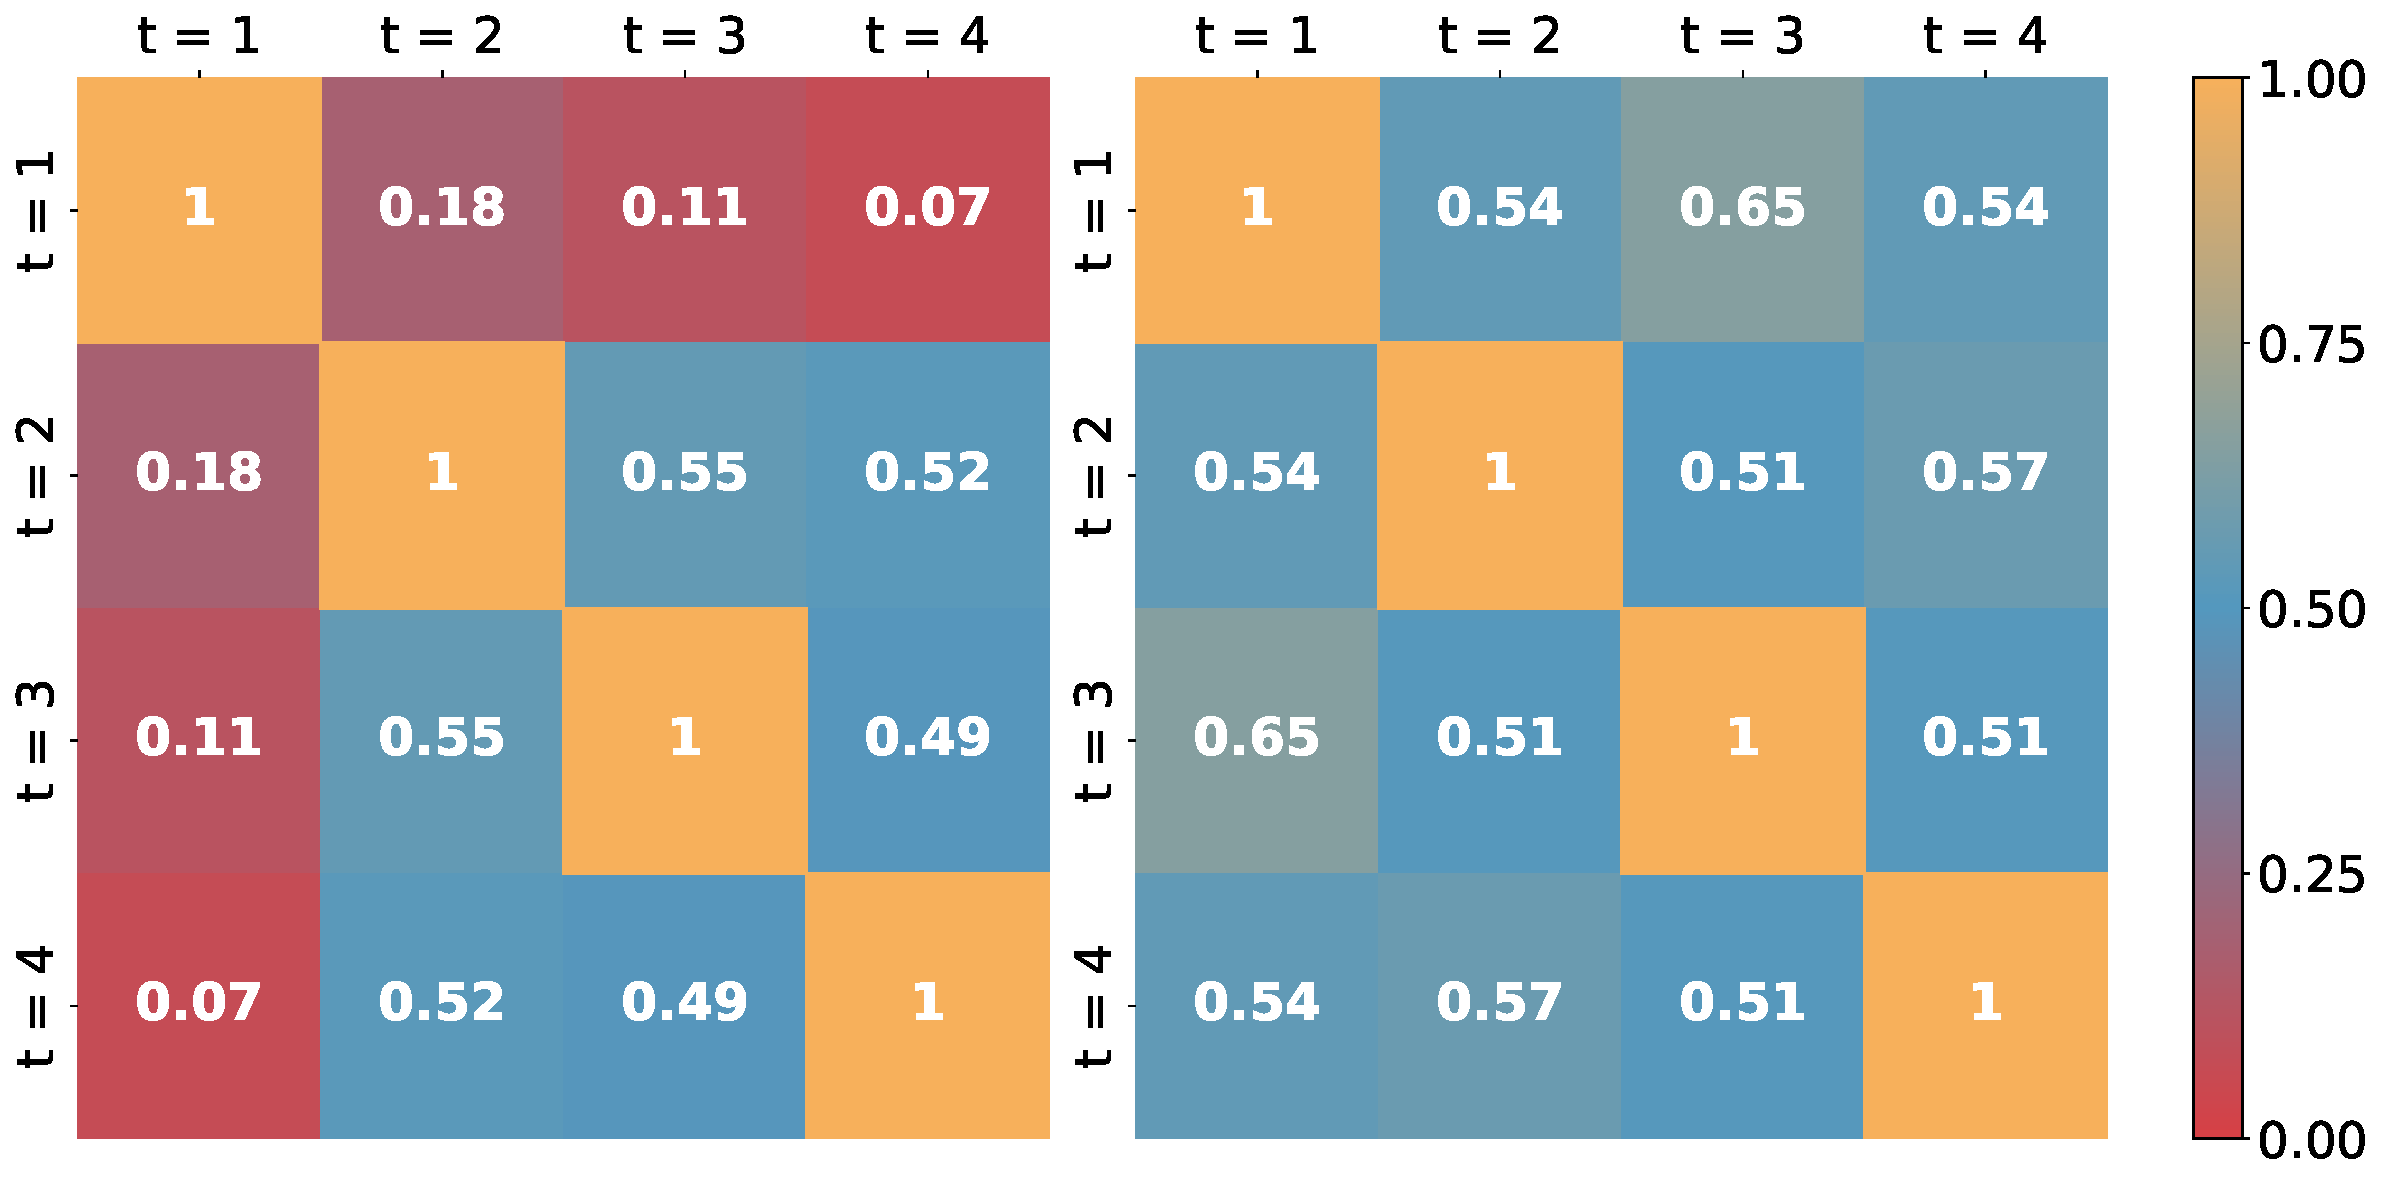
\includegraphics[width=0.99\linewidth]{fig/grad_collision.pdf}
    \caption{\textbf{Gradient conflicts across timesteps with and without MP-Init.} 
We visualize the cosine similarity of gradients across timesteps in ResNet-19 on CIFAR100. 
\emph{Left:} Without MP-Init, the gradient from $t=1$ strongly conflicts with later timesteps, reflecting the temporal inconsistency highlighted by MPS~\cite{ding:2025}. 
\emph{Right:} With MP-Init, conflicts are largely resolved and similarities improve, indicating that MP-Init aligns temporal ensemble members and stabilizes training.}
    \label{fig:gradient_conflict_tcs}
\end{figure}

\subsection{How does MP-Init impact training?}
\label{subsec:how_mpinit}

TEBN~\cite{tebn:2022} and TAB~\cite{tab:2024} have shown that temporal covariate shift (TCS) indeed occurs, and our paper has already demonstrated that MP-Init effectively resolves it. However, prior studies did not provide clear evidence of \emph{how} TCS directly impairs training. Inspired by the ensemble interpretation of SNNs in MPS~\cite{ding:2025}, we revisited this question and conducted an experiment on ResNet-19 with CIFAR100. Specifically, we computed the gradients applied to a given layer at each timestep and measured the cosine similarity across timesteps. As shown in \cref{fig:gradient_conflict_tcs}, without MP-Init (left), the gradients from $t=1$ exhibit strong conflicts with later timesteps, indicating severe inconsistency across the temporal ensemble members. With MP-Init (right), these conflicts are largely alleviated, and the overall cosine similarity improves. This analysis provides the direct evidence that TCS not only degrades inference consistency but also hinders gradient alignment during training, and highlights how MP-Init effectively stabilizes optimization.

\begin{figure}[t]
  \centering
  \begin{subfigure}[b]{0.99\linewidth}
    \centering
    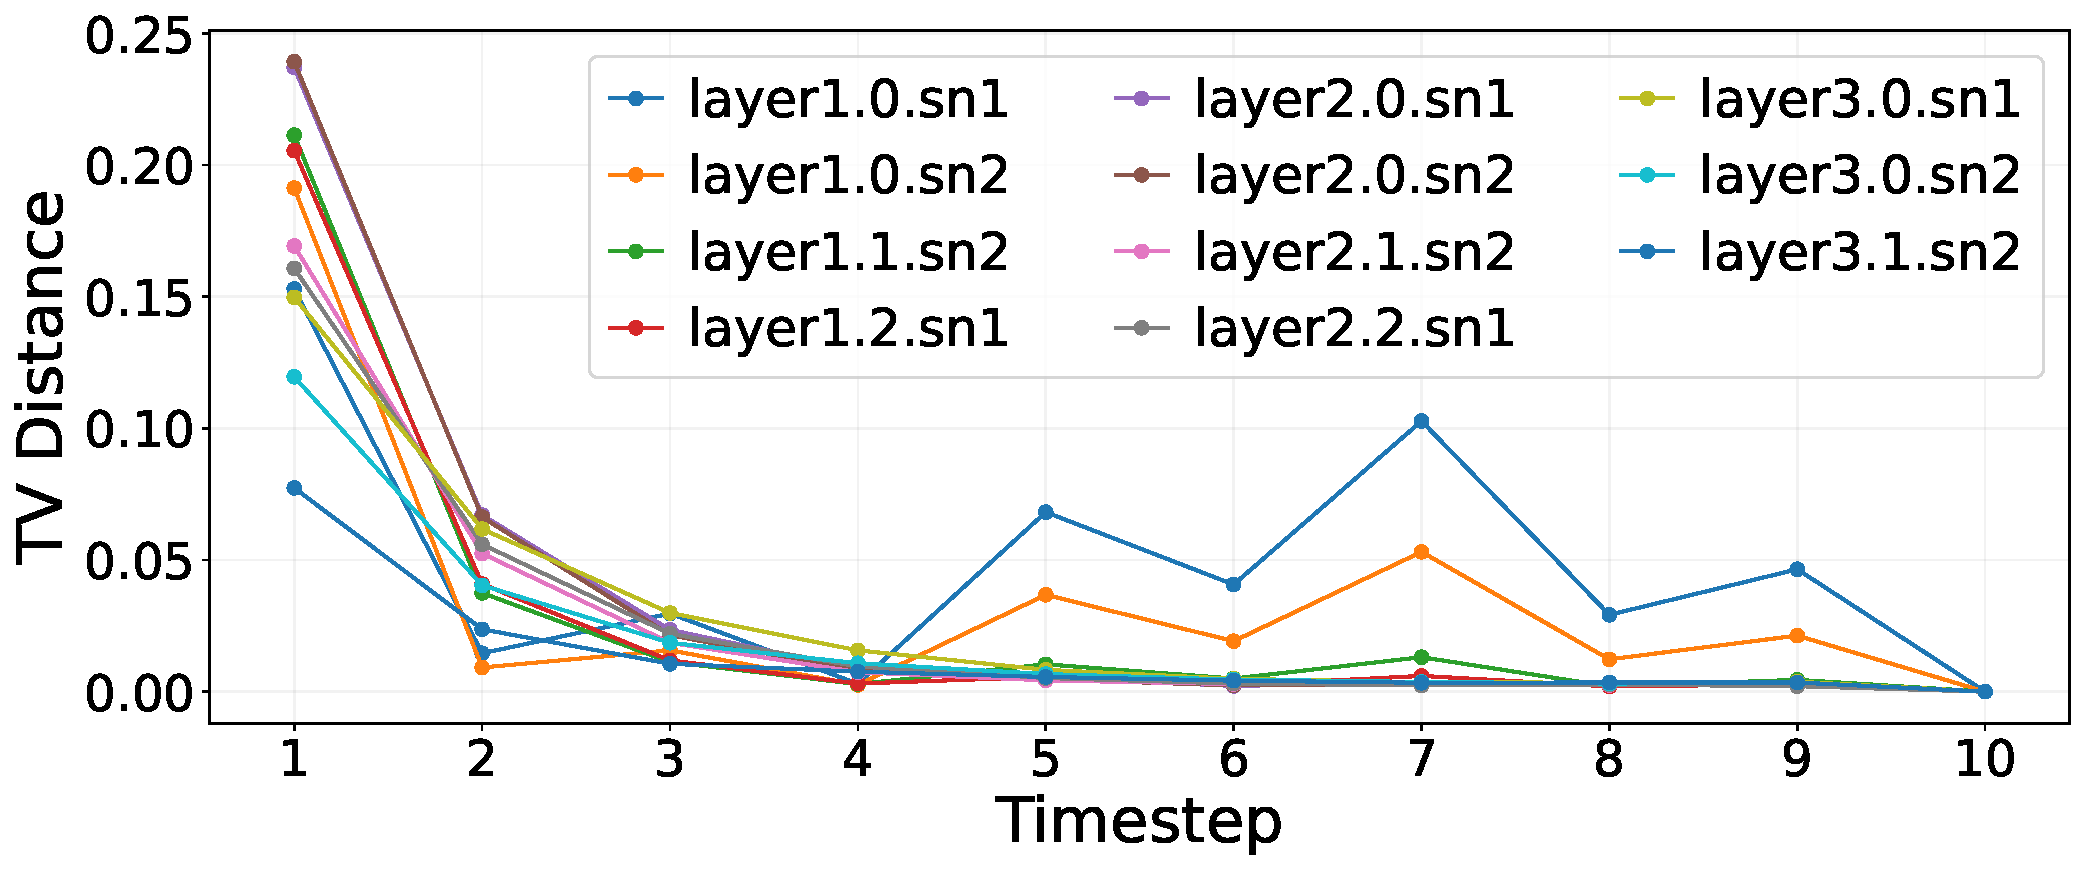
\includegraphics[width=\linewidth]{fig/tv_from_input_distribution.pdf}
    \caption{TV distance between input distributions at different timesteps. Each curve compares $t=1\ldots9$ against the reference at $t=10$.}
    \label{fig:tv-distance}
  \end{subfigure}
  \hfill
  \begin{subfigure}[b]{0.99\linewidth}
    \centering
    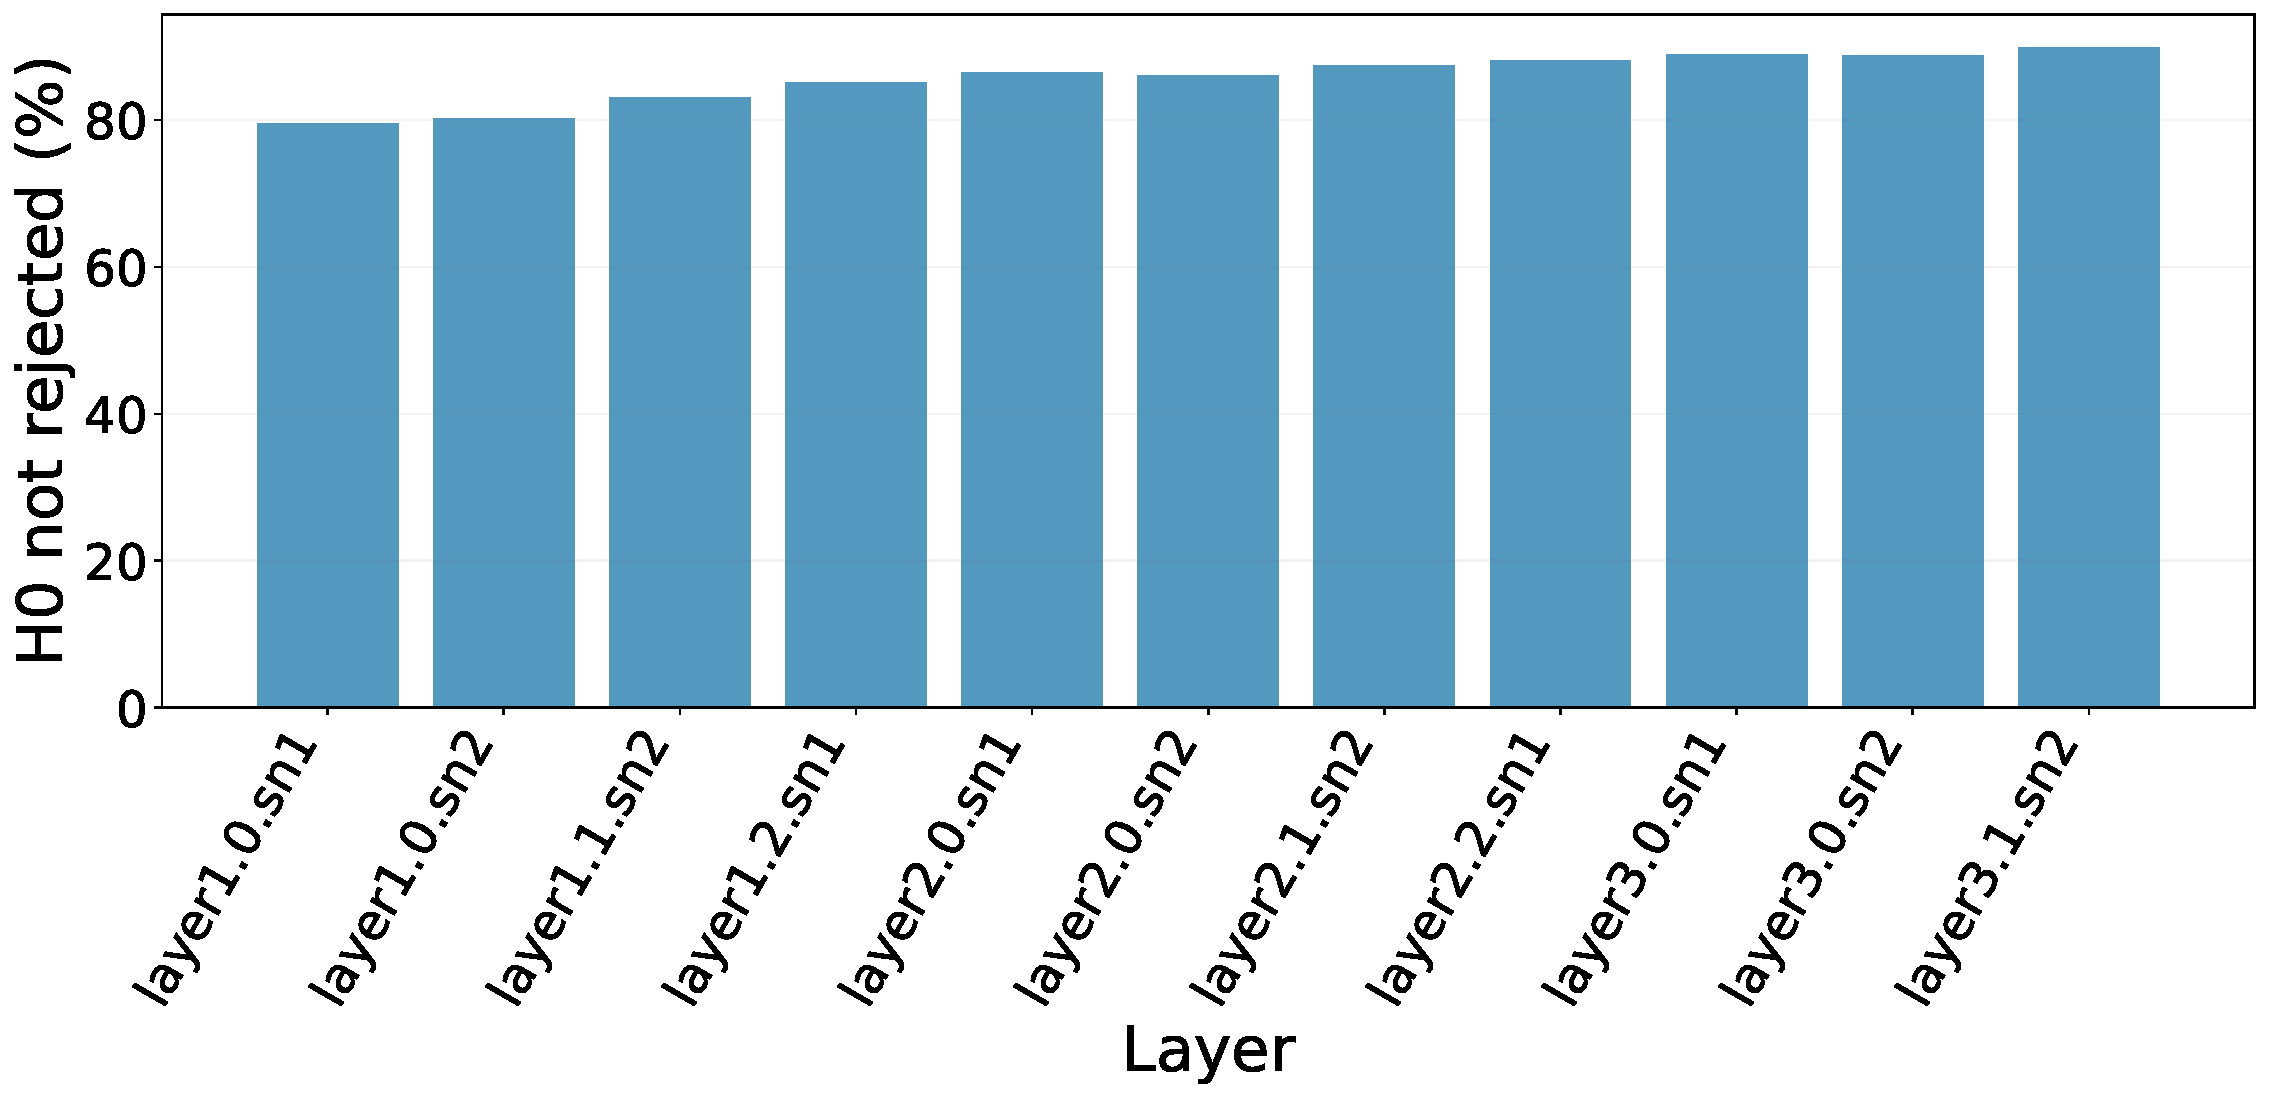
\includegraphics[width=\linewidth]{fig/ljung_box_lag1.pdf}
    \caption{Ljung-Box test at lag=1. Bars show the percentage of neurons for which independence could not be rejected.}
    \label{fig:ljung-box}
  \end{subfigure}
  \hfill
  \begin{subfigure}[b]{0.99\linewidth}
    \centering
    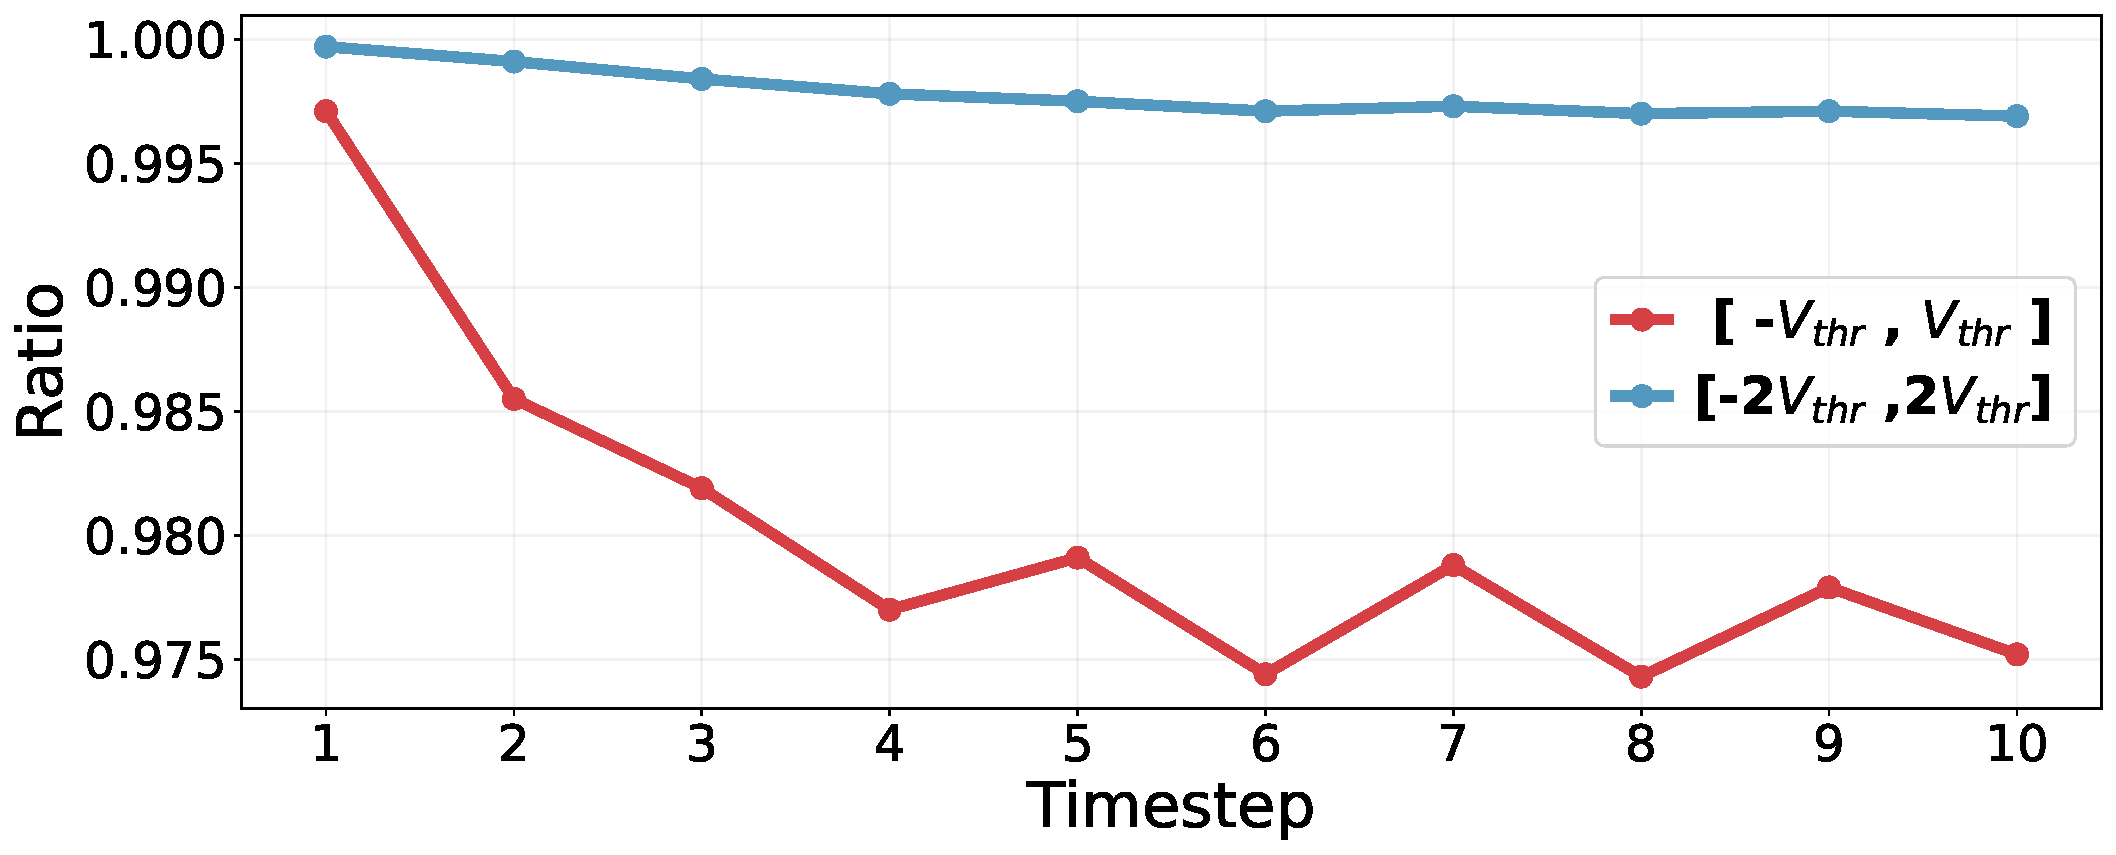
\includegraphics[width=\linewidth]{fig/ratio_ut.pdf}
    \caption{Boundedness ratio of membrane potentials $U[t]$.}
    \label{fig:ratio-bounded}
  \end{subfigure}

  \caption{Empirical validation of Assumption~1 using ResNet-19 trained on \textbf{CIFAR100}. 
  (a) TV distance across timesteps demonstrates near-identical input distributions. 
  (b) Ljung-Box test confirms approximate input independence. 
  (c) Boundedness ratio shows that membrane potentials remain within symmetric ranges relative to the threshold.}
  \label{fig:validation-assumption}
\end{figure}

\subsection{Validation of Assumption 1}
\label{subsec:validation_of_assumption_1}

We empirically verify that inputs are approximately \emph{i.i.d.} and that the membrane potentials of active neurons remain bounded, in line with Assumption~1. Using a trained ResNet-19 on CIFAR100, we report three complementary metrics:

\begin{itemize}
    \item \textbf{Identical distribution (\cref{fig:tv-distance}).} We compute the TV distance between input distributions at timesteps $t=1\ldots9$ and the reference at $t=10$. Distances are consistently small ($<0.1$ after $t=2$), indicating that the distribution quickly stabilizes and remains nearly identical across timesteps.
    \item \textbf{Independence (\cref{fig:ljung-box}).} We applied the Ljung-Box test for autocorrelation with significance level $\alpha=0.05$ using $\text{lag}=1$. It illustrates 80--90\% of neurons do not reject $H_0$ (independence). This suggests that temporal correlations are minor, supporting practical independence.
    \item \textbf{Boundedness (\cref{fig:ratio-bounded}).} Over 97\% of membrane potentials remain within $\pm V_{\text{thr}}$ at all timesteps, and nearly all values lie within $\pm 2V_{\text{thr}}$, confirming that the dynamics are effectively bounded in practice.
\end{itemize}

Taken together, these results confirm that Assumption~1 holds empirically: the inputs to spiking layers are nearly i.i.d., and the membrane potentials of active neurons remain bounded, thereby validating the theoretical conditions. Consistent findings are observed on DVS-CIFAR10 as well, as shown in \cref{fig:validation-assumption-dvs}, where ResNet-19 exhibits the same behavior satisfying all parts of Assumption~1.

\begin{figure}[h]
  \centering
  \begin{subfigure}[b]{0.99\linewidth}
    \centering
    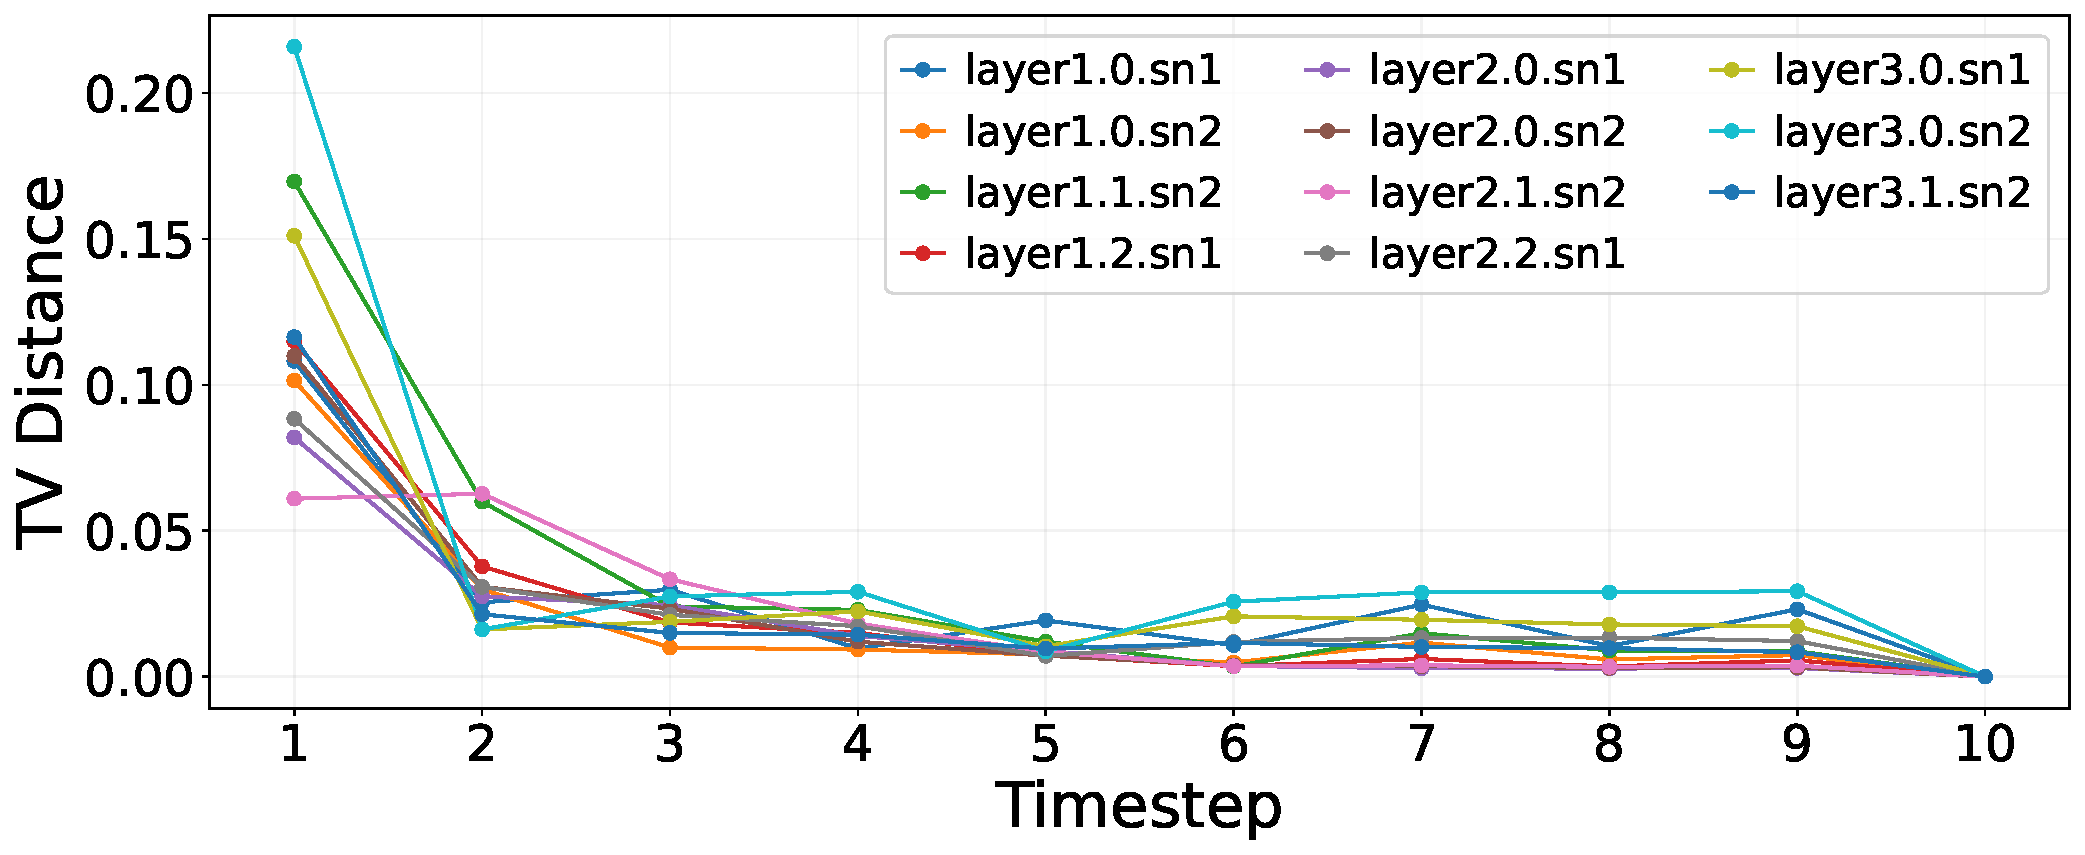
\includegraphics[width=\linewidth]{fig/tv_from_input_distribution_dvs.pdf}
    \caption{TV distance between input distributions at different timesteps. Each curve compares $t=1\ldots9$ against the reference at $t=10$.}
    \label{fig:tv-distance-dvs}
  \end{subfigure}
  \hfill
  \begin{subfigure}[b]{0.99\linewidth}
    \centering
    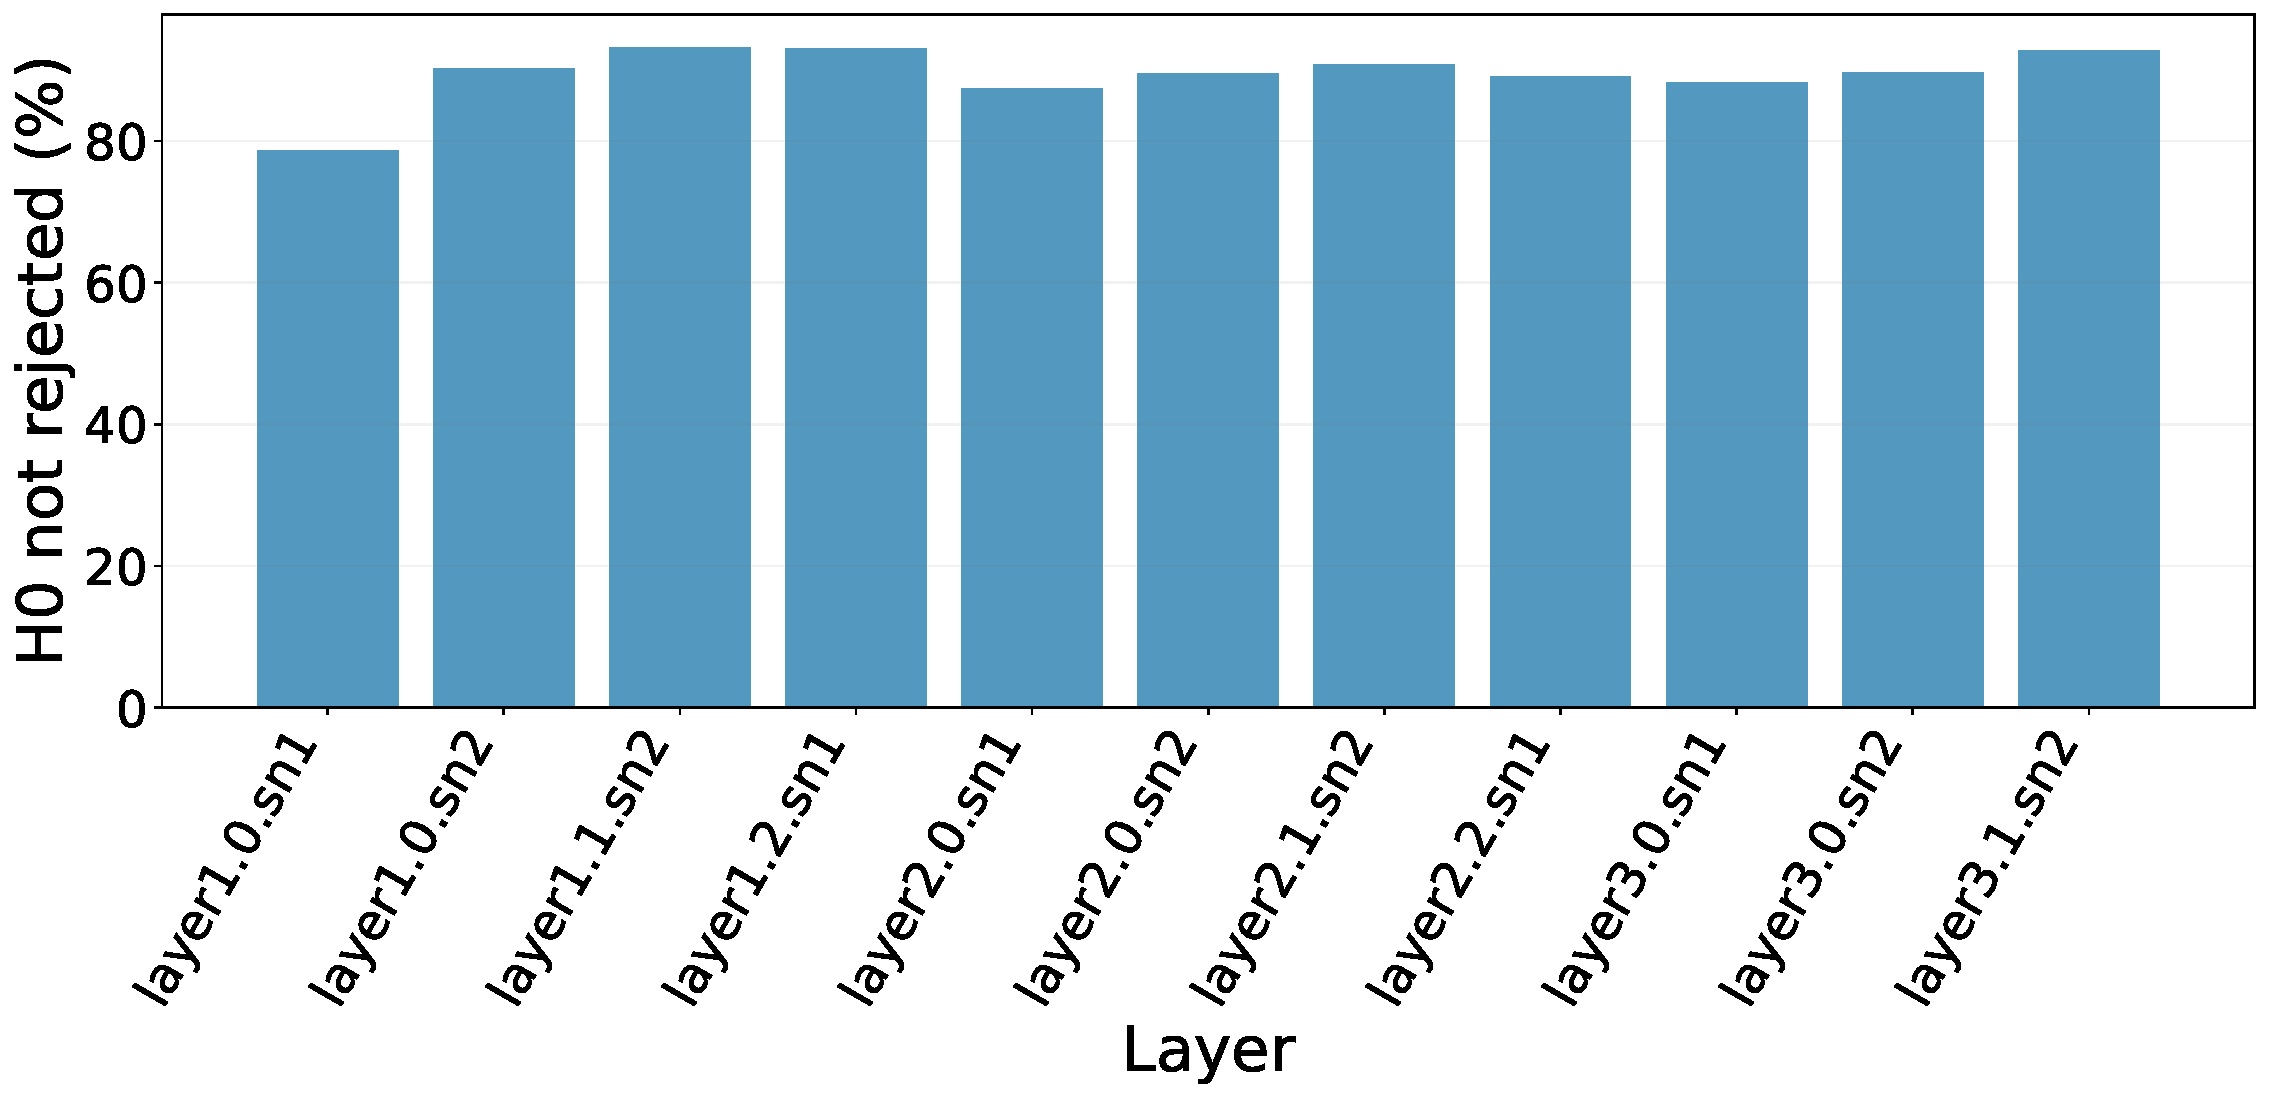
\includegraphics[width=\linewidth]{fig/ljung_box_lag1_dvs.pdf}
    \caption{Ljung-Box test at lag=1. Bars show the percentage of neurons for which independence could not be rejected.}
    \label{fig:ljung-box-dvs}
  \end{subfigure}
  \hfill
  \begin{subfigure}[b]{0.99\linewidth}
    \centering
    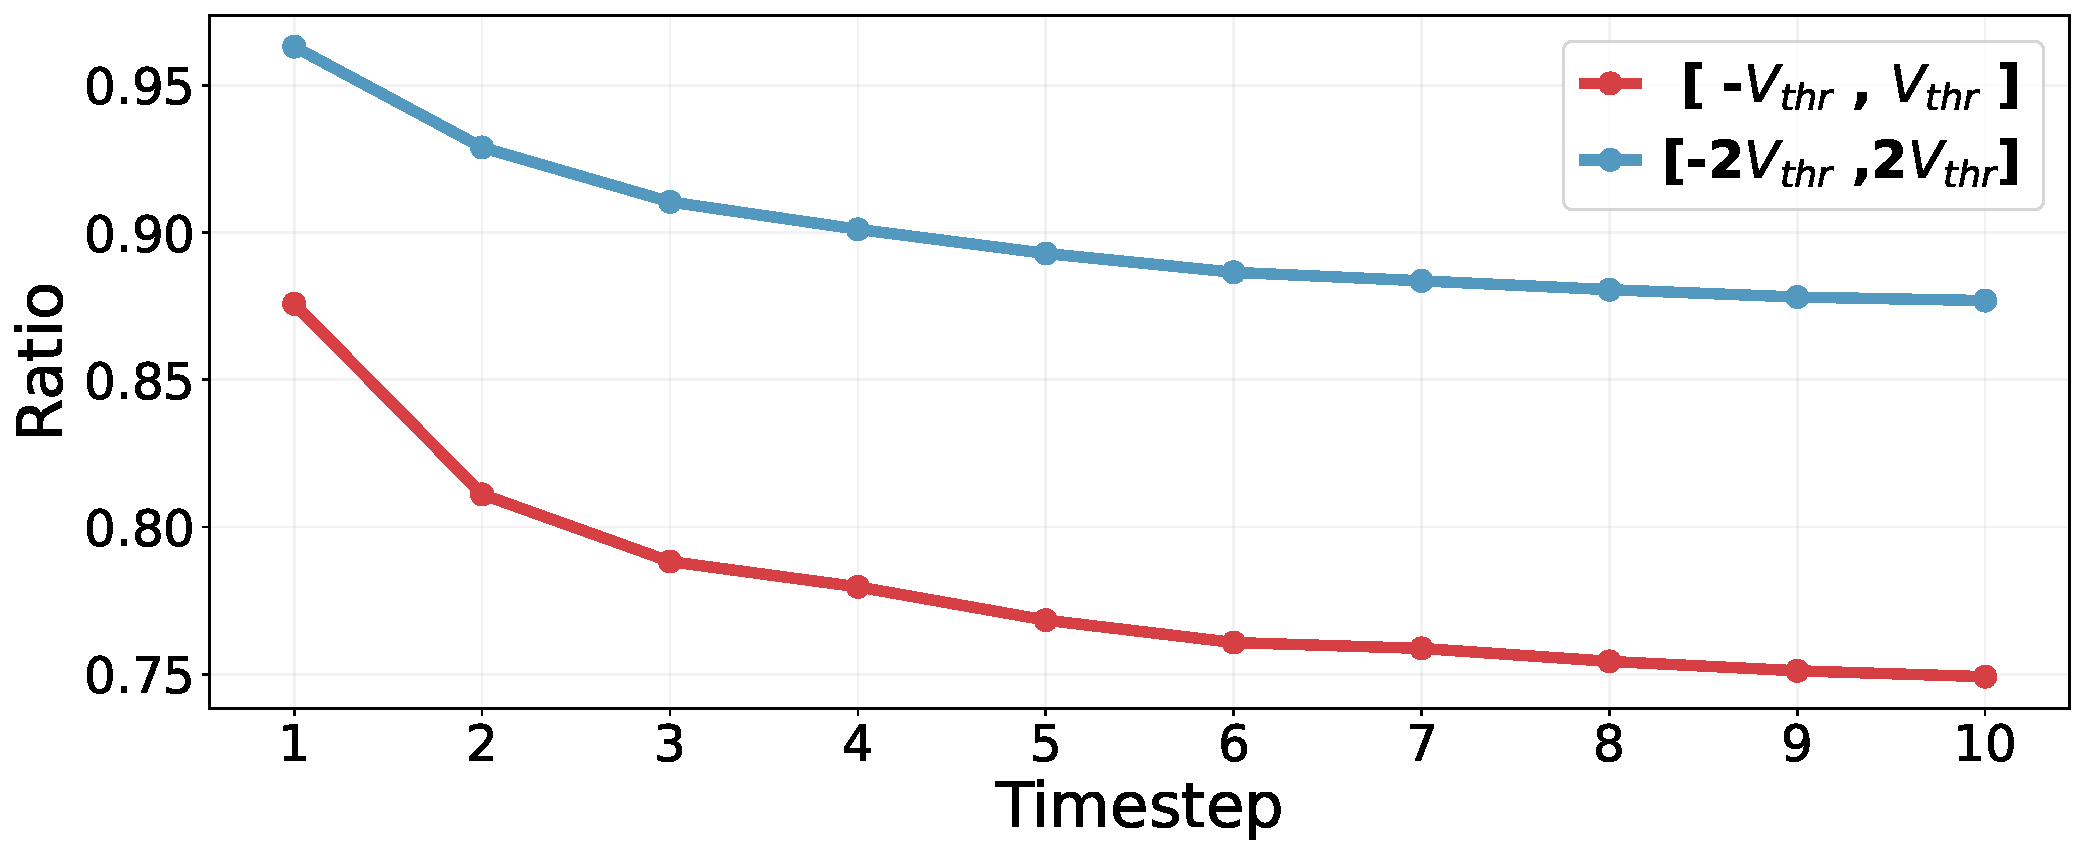
\includegraphics[width=\linewidth]{fig/ratio_ut_dvs.pdf}
    \caption{Boundedness ratio of membrane potentials $U[t]$.}
    \label{fig:ratio-bounded-dvs}
  \end{subfigure}

  \caption{Empirical validation of Assumption~1 using ResNet-19 trained on \textbf{DVS-CIFAR10}. 
  (a) TV distance across timesteps demonstrates near-identical input distributions. 
  (b) Ljung-Box test confirms approximate input independence. 
  (c) Boundedness ratio shows that membrane potentials remain within symmetric ranges relative to the threshold.}
  \label{fig:validation-assumption-dvs}
\end{figure}

\begin{figure}[h]
  \centering
  \begin{subfigure}[b]{0.99\linewidth}
    \centering
    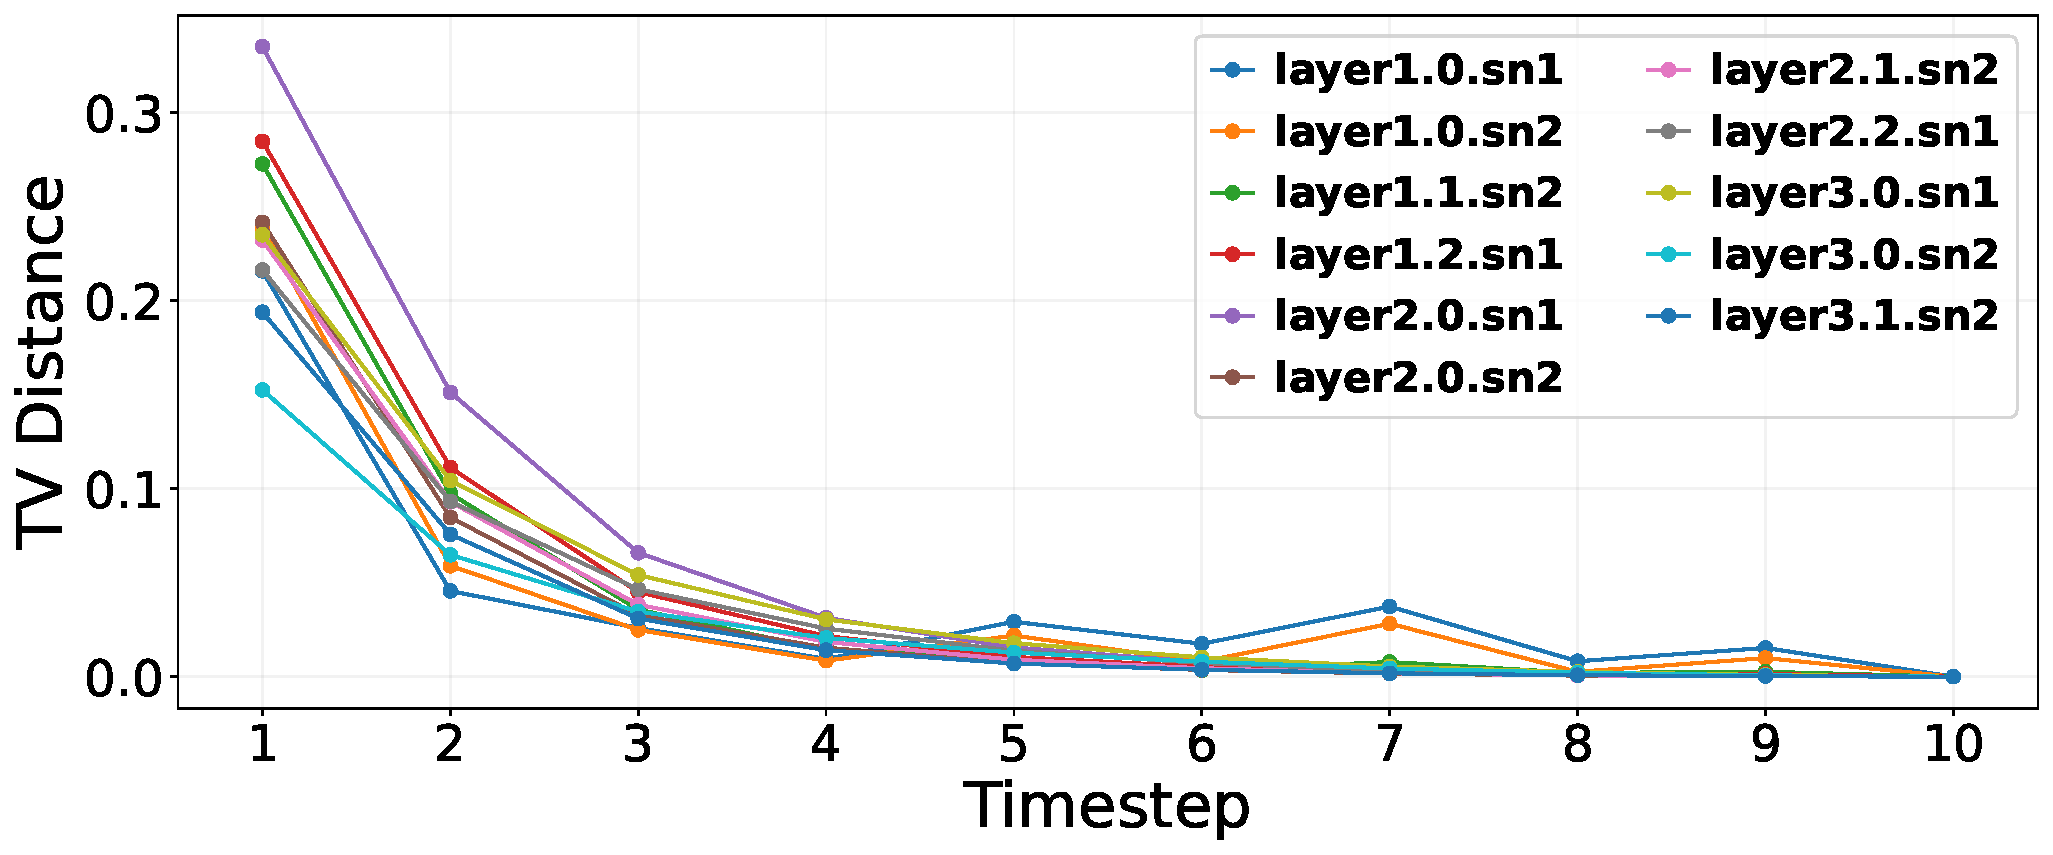
\includegraphics[width=\linewidth]{fig/tv_distance.pdf}
    \caption{CIFAR100 (ResNet-19).}
    \label{fig:tv-mp-convergence-distance-cifar100}
  \end{subfigure}
  \hfill
  \begin{subfigure}[b]{0.99\linewidth}
    \centering
    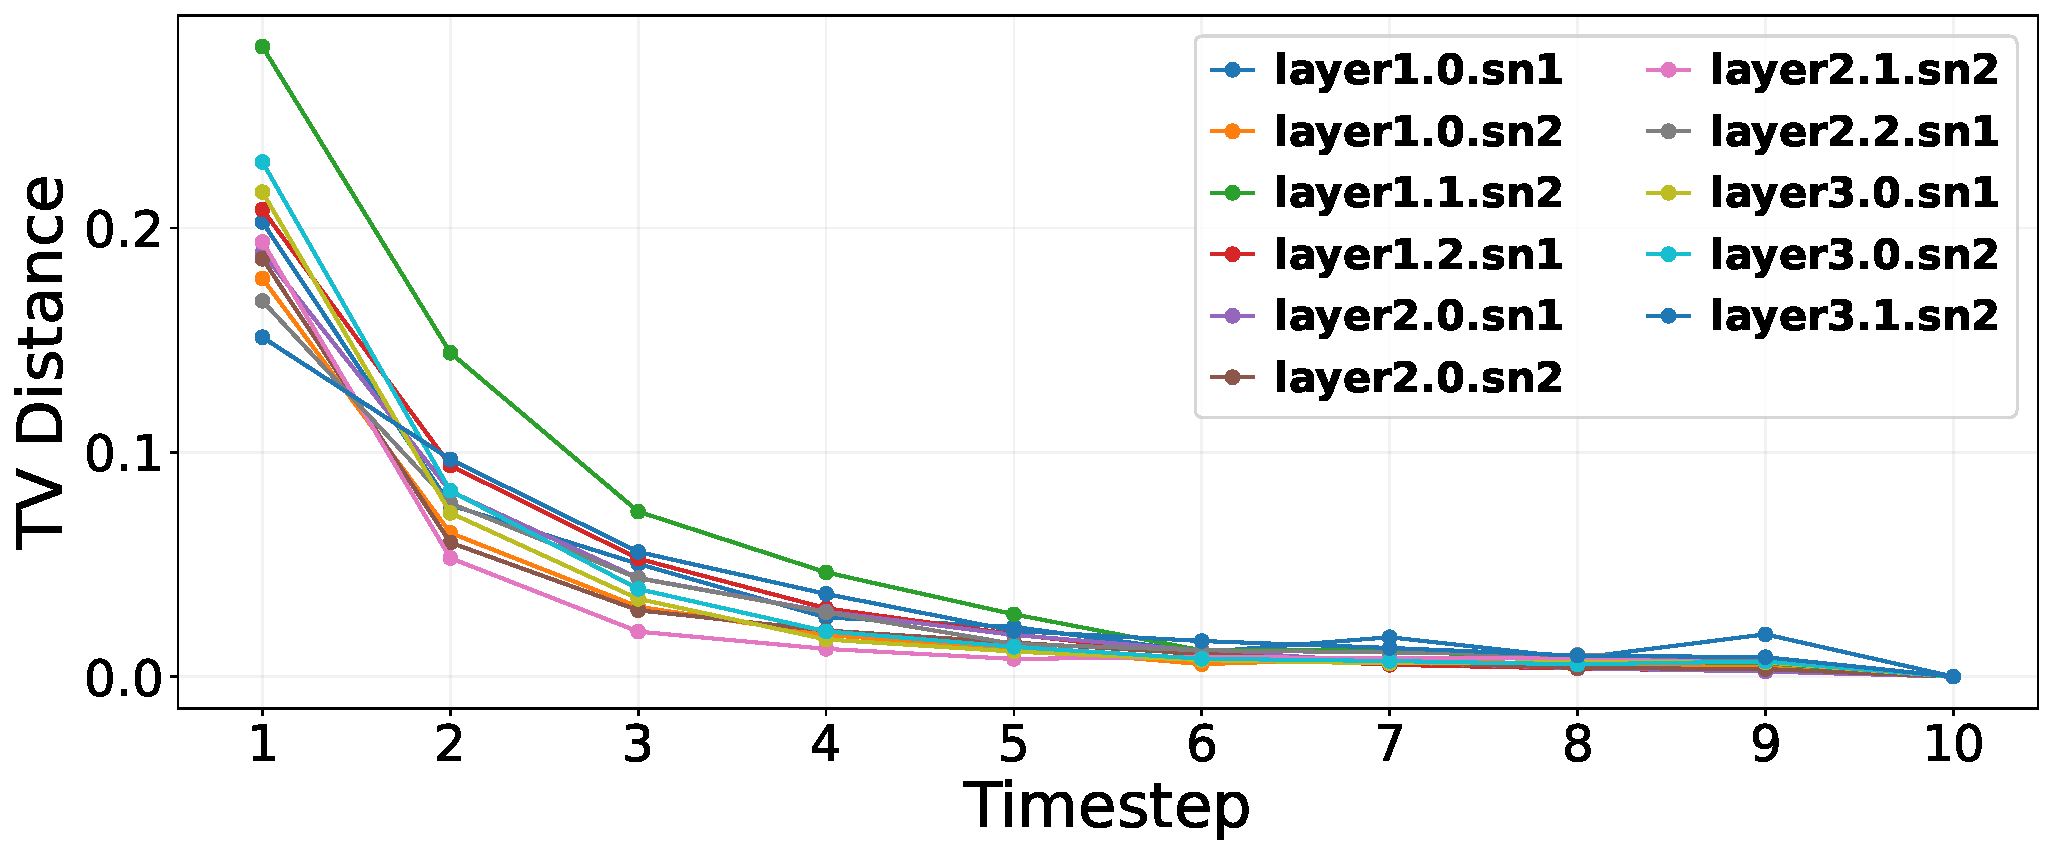
\includegraphics[width=\linewidth]{fig/tv_distance_dvs.pdf}
    \caption{DVS-CIFAR10 (ResNet-19).}
    \label{fig:tv-mp-convergence-distance-dvs}
  \end{subfigure}
  \caption{TV distance between membrane potentials $U^l[t]$ at each timestep and the reference at $t=10$. Across both CIFAR100 and DVS-CIFAR10, TV distance is initially large ($>0.3$ at $t=1$) but decreases sharply by $t=2$, and falls below $0.1$ by $t=3$, indicating rapid convergence of membrane dynamics.}
  \label{fig:tv-distance-convergence}
\end{figure}

\begin{table}[h]
\centering
\small
\begin{tabular}{lcc}
\toprule
\textbf{Method} & \textbf{w/o MP-Init (\%)} & \textbf{w/ MP-Init (\%)} \\
\midrule
tdBN (timestep=2) & 72.35 $\pm$ 0.18 & \textbf{74.01 $\pm$ 0.33} \\
\bottomrule
\end{tabular}
\caption{Effect of MP-Init at early timesteps on CIFAR100 using ResNet-19}
\label{tab:convergence-mpinit}
\end{table}

\subsection{Convergence of Membrane Potentials}
\label{subsec:convergence_speed}

As predicted by Theorem~1, the empirical TV distance curves in \cref{fig:tv-distance-convergence} clearly exhibit \emph{exponential convergence}: deviations are large at $t=1$ but shrink rapidly, already becoming negligible ($<0.1$) by $t=3$. This rapid convergence is highly desirable for SNNs, since reducing the number of timesteps directly improves both energy efficiency and latency. Notably, the benefit is especially pronounced at very low timesteps: at timestep=2, MP-Init delivers a \textbf{1.66\%pt} accuracy improvement over the baseline (\cref{tab:convergence-mpinit}), highlighting that our method enables reliable inference even under aggressive latency constraints.


\subsection{Proof of Theorem 1}
\label{subsec:proof_of_theorem_1}
\textbf{Theorem 1.}
Under Assumption 1, the sequence $\{U[t]\}_{t \ge 0}$ forms a Markov chain with transition kernel $P$. This chain satisfies Doeblin’s minorization condition, ensuring the existence of a unique stationary distribution $\pi$. Moreover, the TV distance between $U[t]$ and $\pi$ decreases exponentially.

\medskip
\noindent
\textbf{Step 1: Markov Property}

We begin by confirming that \( \{U[t]\}_{t \geq 0} \) forms a Markov chain. The dynamics of \( U[t] \) are given by:
\begin{equation}
    U[t+1] = f(U[t], I_{in}[t+1]),
\end{equation}
where \( f(\cdot) \) is a deterministic function dependent on the current membrane potential \( U[t] \) and the new input \( I_{in}[t+1] \). Since the inputs \( \{I_{in}[t]\}_{t \geq 0} \) follow i.i.d, the future state \( U[t+1] \) depends solely on the current state \( U[t] \) and not on any earlier states.

Thus, the probability of transitioning to \( U[t+1] \) given the entire history \( \{U[s]\}_{s \leq t} \) depends only on \( U[t] \):
\begin{equation}
    P(U[t+1] \in A \mid U[t], \dots, U[0]) = P(U[t+1] \in A \mid U[t]),
\end{equation}
which confirms that \( \{U[t]\}_{t \geq 0} \) is indeed a Markov chain.

\medskip
\noindent
\textbf{Step 2: The Transition Kernel \( P(x, A) \) and Its Relation} % to \( U[t] \) and \( U[t+1] \)}

The transition kernel \( P(x, A) \) describes the probability of moving from state \( x \) at time \( t \) to the set \( A \) at time \( t+1 \). Specifically, for the Markov chain \( \{U[t]\}_{t \geq 0} \), \( P(x, A) \) is the probability that the membrane potential at time \( t+1 \), denoted by \( U[t+1] \), falls within the set \( A \) given that the membrane potential at time \( t \) is \( U[t] = x \). This is formulated as:
\begin{equation}
    P(x, A) = P(U[t+1] \in A \mid U[t] = x).
\end{equation}

The transition kernel can be represented using the transition density \( p(x, y) \), which is the probability density function for transitioning from state \( x \) to state \( y \):
\begin{equation}
    P(x, A) = \int_A p(x, y) dy,
\end{equation}
where \( p(x, y) \) encapsulates the dynamics governed by the function \( f(U[t], I_{in}[t+1]) \) and the input \( I_{in}[t+1] \).

\medskip
\noindent
\textbf{Step 3: Doeblin's Minorization Condition}

We now show that the Markov chain \( \{U[t]\}_{t \geq 0} \) satisfies the Doeblin's minorization condition~\cite{rosenthal:1995}. We need to demonstrate the existence of a constant \( \epsilon > 0 \) and a probability measure \( \mu(\cdot) \) such that for any \( x \in S \) and any measurable set \( A \subseteq S \), the transition probability satisfies:
\begin{equation}
\label{eq:minimorization_condition}
    P(x, A) \geq \epsilon \mu(A).
\end{equation}

Given that the state space \( S \) is bounded by \( [u^{-}, u^{+}] \), and assuming the transition density \( p(x, y) \) is smooth and continuous (as the inputs are i.i.d. Gaussian), there exists a positive lower bound \( \delta \) for \( p(x, y) \) over the state space \( S \). This implies that for any measurable set \( A \subseteq S \):
\begin{equation}
    P(x, A) = \int_A p(x, y) dy \geq \delta \cdot \mu(A),
\end{equation}
where \( \mu(\cdot) \) is a probability measure (e.g., uniform measure) over \( S \). Setting \( \epsilon = \delta \), we can validate that \cref{eq:minimorization_condition} is satisfied.

\medskip
\noindent
\textbf{Step 4: Exponential Decrease in TV Distance}

As a result of the Doeblin's minorization condition, the TV distance between the distribution \( P^n(x, \cdot) \) of the Markov chain after \( n \) steps, starting from any state \( x \), and the stationary distribution \( \pi(\cdot) \) satisfies:
\begin{equation}
\label{eq:convergence_speed}
    \| P^n(x, \cdot) - \pi(\cdot) \|_{TV} \leq C(1 - \epsilon)^n,
\end{equation}
for some constant \( C > 0 \). This inequality shows that the TV distance decreases exponentially as \( n \) increases, implying that the Markov chain converges rapidly to the stationary distribution \( \pi \). This also implies the uniqueness and existence of the stationary distribution.

\subsection{Proof of Lemma 1}
\label{subsec:proof_of_lemma_1}
\textbf{Lemma 1.} Among all constants \( c \in \mathbb{R} \), \( c = E[\pi] \) minimizes expected square difference \(E[(\pi-c)^{2}]\).

\medskip

We begin by calculating the expected value of the L2 norm between \( U^{*} \) and a constant \( c \):

\begin{equation}
    E[|U^{*} - c|^{2}] = E[(U^{*} - c)^{2}] = E[U^{*2}] - 2E[U^{*}]c + c^2.
\end{equation}

Next, we take the derivative of this expression with respect to \( c \):

\begin{equation}
    \frac{\partial E[|U^{*} - c|^{2}]}{\partial c} = -2E[U^{*}] + 2c.
\end{equation}

Setting the derivative to zero to find the minimum, we obtain:

\begin{equation}
    c = E[U^{*}].
\end{equation}

Thus, the L2 norm is minimized when \( c = E[U^{*}] \), proving the lemma.


\section{Additional Details: TrSG}
\label{sec:appendix_trsg}

\subsection{How does TrSG impact training?}
\label{subsec:how_trsg_impacts_training}

\paragraph{Protocol.}
We analyze gradient flow of ResNet-19 on CIFAR100 with $\text{timestep}{=}4$ for 200 epochs. To isolate the effect of the SG formulation, we \emph{fix} $\tau{=}2.0$ and do not train $V_{\text{thr}}$ or $\tau$. We use a rectangular surrogate with $\gamma{=}1$ and the soft-reset mechanism.

\paragraph{Metrics.}
We quantify stability with three complementary metrics computed on convolutional weights of a given layer:
\[
\text{AbsStr}=\operatorname*{mean}_i |g_i|,\quad
\]
\[
\text{RatioAG}=\frac{1}{N}\sum_i \mathds{1}\!\left(|x_i|<\tfrac{\gamma}{2}\right),\quad
\]
\[
\text{GradCV}=\frac{\operatorname{std}_i(|g_i|)}{\operatorname*{mean}_i(|g_i|)},
\]
where $g_i=\partial \mathcal{L}/\partial W_i$ and $x_i$ is the surrogate argument. 

\textbf{AbsStr} measures the average gradient magnitude. Very low values indicate vanishing gradients, where updates stall, 
while excessively high values point to exploding gradients, leading to erratic updates. 
Stable training requires AbsStr to remain in a moderate range. 
\textbf{RatioAG} quantifies the fraction of neurons receiving nonzero gradients. 
If RatioAG is too low, most neurons fail to receive updates (gradient starvation); 
if too high, too many neurons receive updates, causing gradient flood and poor selectivity. 
An intermediate range is thus ideal. 

\textbf{GradCV} captures the variability of gradient magnitudes. 
Low variance (CV $<1$) implies smooth, balanced updates that can be handled by a single learning rate, 
whereas high variance (CV $\gg 1$) means some weights update disproportionately faster than others, destabilizing training.  
TrSG is designed to maintain AbsStr at moderate levels, keep RatioAG in the healthy range, 
and reduce GradCV, together ensuring stable optimization.

\paragraph{Reference case ($V_{\text{thr}}{=}1.0$,~\cref{tab:metrics_ref}).}
This widely used threshold serves as a baseline where all SG variants behave same (though $1.0$ is not necessarily optimal). From epoch 1 to 100 we observe steadily improving yet stable gradients.

\begin{table}[t]
\centering
\small
\begin{tabular}{ccccc}
\toprule
\textbf{Epoch} & \textbf{$V_{\text{thr}}{=}1.0$} & \textbf{AbsStr} & \textbf{RatioAG (\%)} & \textbf{GradCV} \\
\midrule
1   & any SG & 0.0122 & 6.72  & 0.818 \\
100 & any SG & 0.0211 & 18.97 & 0.571 \\
\bottomrule
\end{tabular}
\caption{Reference case where all SG variants behave same (ResNet‑19, CIFAR100, $\text{timestep}{=}4$, $\tau{=}2.0$).}
\label{tab:metrics_ref}
\end{table}

\paragraph{Low threshold ($V_{\text{thr}}{=}0.1$,~\cref{tab:metrics_low}).}
This stress test exposes small-threshold failure modes. At epoch 1, AS‑SG floods (wide window), RS‑SG explodes due to the $1/V_{\text{thr}}$ factor, while TrSG remains stable. By epoch 100, AS‑SG still shows instability and RS‑SG diverges; TrSG trains smoothly. These trends align with accuracy outcomes in \cref{tab:no_training_results}.

\begin{table}[t]
\centering
\small
\begin{tabular}{ccccc}
\toprule
\textbf{Epoch} & \textbf{$V_{\text{thr}}{=}0.1$} & \textbf{AbsStr} & \textbf{RatioAG (\%)} & \textbf{GradCV} \\
\midrule
\multirow{3}{*}{1}   & AS-SG & 0.2756 & 31.25 & 5.01  \\
& RS-SG & 7.8191 & 0.01  & 37.11 \\
& TrSG  & 0.0046 & 3.05  & \textbf{0.861} \\
\addlinespace[2pt]
\midrule
\multirow{3}{*}{100} & AS-SG & 0.0145 & 90.20 & 1.22  \\
& RS-SG & NaN    & 0.00  & NaN   \\
& TrSG  & 0.0153 & 21.45 & \textbf{0.865} \\
\bottomrule
\end{tabular}
\caption{Low‑threshold stress test (CIFAR100, $\text{timestep}{=}4$, $\tau{=}2.0$). RS‑SG explodes (diverges), AS‑SG floods, while TrSG remains stable. See \cref{tab:no_training_results} for accuracy.}
\label{tab:metrics_low}
\end{table}

\paragraph{High threshold ($V_{\text{thr}}{=}2.0$,~\cref{tab:metrics_high}).}
Here the absolute window of AS‑SG is too narrow and RS‑SG’s $1/V_{\text{thr}}$ suppresses signals. AS‑SG starves, RS‑SG vanishes with high variance, while TrSG stays trainable. The accuracy pattern is consistent with \cref{tab:no_training_results}.

\begin{table}[t]
\centering
\small
\begin{tabular}{ccccc}
\toprule
\textbf{Epoch} & \textbf{$V_{\text{thr}}{=}2.0$} & \textbf{AbsStr} & \textbf{RatioAG (\%)} & \textbf{GradCV} \\
\midrule
\multirow{3}{*}{1} & AS-SG & 0.0058 & 0.78 & 17.14 \\
& RS-SG & 0.0066 & 1.64 & 0.639 \\
& TrSG  & 0.0092 & 1.62 & \textbf{0.961} \\
\midrule
\addlinespace[2pt]
\multirow{3}{*}{100} & AS-SG & 0.0000 & 0.00 & 0.000 \\
& RS-SG & 0.0021 & 0.10 & 2.247 \\
& TrSG  & 0.0323 & 6.90 & \textbf{0.731} \\
\bottomrule
\end{tabular}
\caption{High‑threshold stress test (CIFAR100, $\text{timestep}{=}4$, $\tau{=}2.0$). AS‑SG starves, RS‑SG vanishes, TrSG preserves stable updates. See \cref{tab:no_training_results} for accuracy.}
\label{tab:metrics_high}
\end{table}

\begin{table}[t]
\centering
\small
\begin{tabular}{cc|ccccc}
\toprule
\textbf{Reset} & \textbf{SG} & \multicolumn{4}{c}{\(\boldsymbol{V_{\text{thr}}}\)} \\
\cmidrule(lr){3-7}
\multicolumn{2}{c|}{} & 0.1 & 0.5 & 1.0 & 1.5 & 2.0 \\
\midrule
\multirow{3}{*}{\textbf{Soft}} 
  & AS-SG        & 61.59 & 75.96 & ---  & 69.97  & 18.09 \\
  & RS-SG        & \emph{div.} & 76.12 & ---   & 71.43  & 5.43 \\
  & \textbf{TrSG}  & \textbf{73.99} & \textbf{76.82} & \textbf{75.56} & \textbf{71.97}  & \textbf{64.27} \\
\midrule
\multirow{3}{*}{\textbf{Hard}} 
  & AS-SG        & 67.71   & \textbf{76.34} & ---   & 68.42  & 12.27 \\
  & RS-SG        & 10.36   & 75.85 & ---   & 72.51  & 52.10 \\
  & \textbf{TrSG}  & \textbf{68.94}   & 76.33 & \textbf{75.72} & \textbf{73.86}  & \textbf{68.42} \\
\bottomrule
\end{tabular}
\caption{
Accuracy (\%) with fixed $\tau{=}2.0$ and \emph{frozen} $V_{\text{thr}}$ and $\tau$ to isolate SG effects. 
We vary $V_{\text{thr}}\!\in\!\{0.1,0.5,1.0,1.5,2.0\}$ under soft/hard resets. 
Conventional SGs fail outside a narrow range (explosion at $0.1$, starvation/vanishing at $2.0$), while \textbf{TrSG} remains robust across thresholds.}
\label{tab:no_training_results}
\end{table}

\paragraph{Do real trainings visit such extreme thresholds?}
Yes. When $V_{\text{thr}}$ is trainable, many layers drift toward \emph{lower} thresholds (often $\ll1$), while late/deep layers move \emph{upward} toward larger values (around $\sim 2$ on CIFAR100 and even higher on ImageNet). 
\Cref{fig:vthr_dynamics} summarizes these trajectories: CIFAR100 and DVS-CIFAR10 show several early layers decreasing below $1$ and the last layer increasing, whereas ImageNet exhibits a wider spread with some deep layers rising well beyond $2$. 
These observations confirm that the brittle regimes identified for AS-SG/RS-SG are indeed encountered during training, precisely where TrSG’s threshold-robustness is most beneficial.


\begin{figure}[h]
  \centering
  \begin{subfigure}[b]{0.99\linewidth}
    \centering
    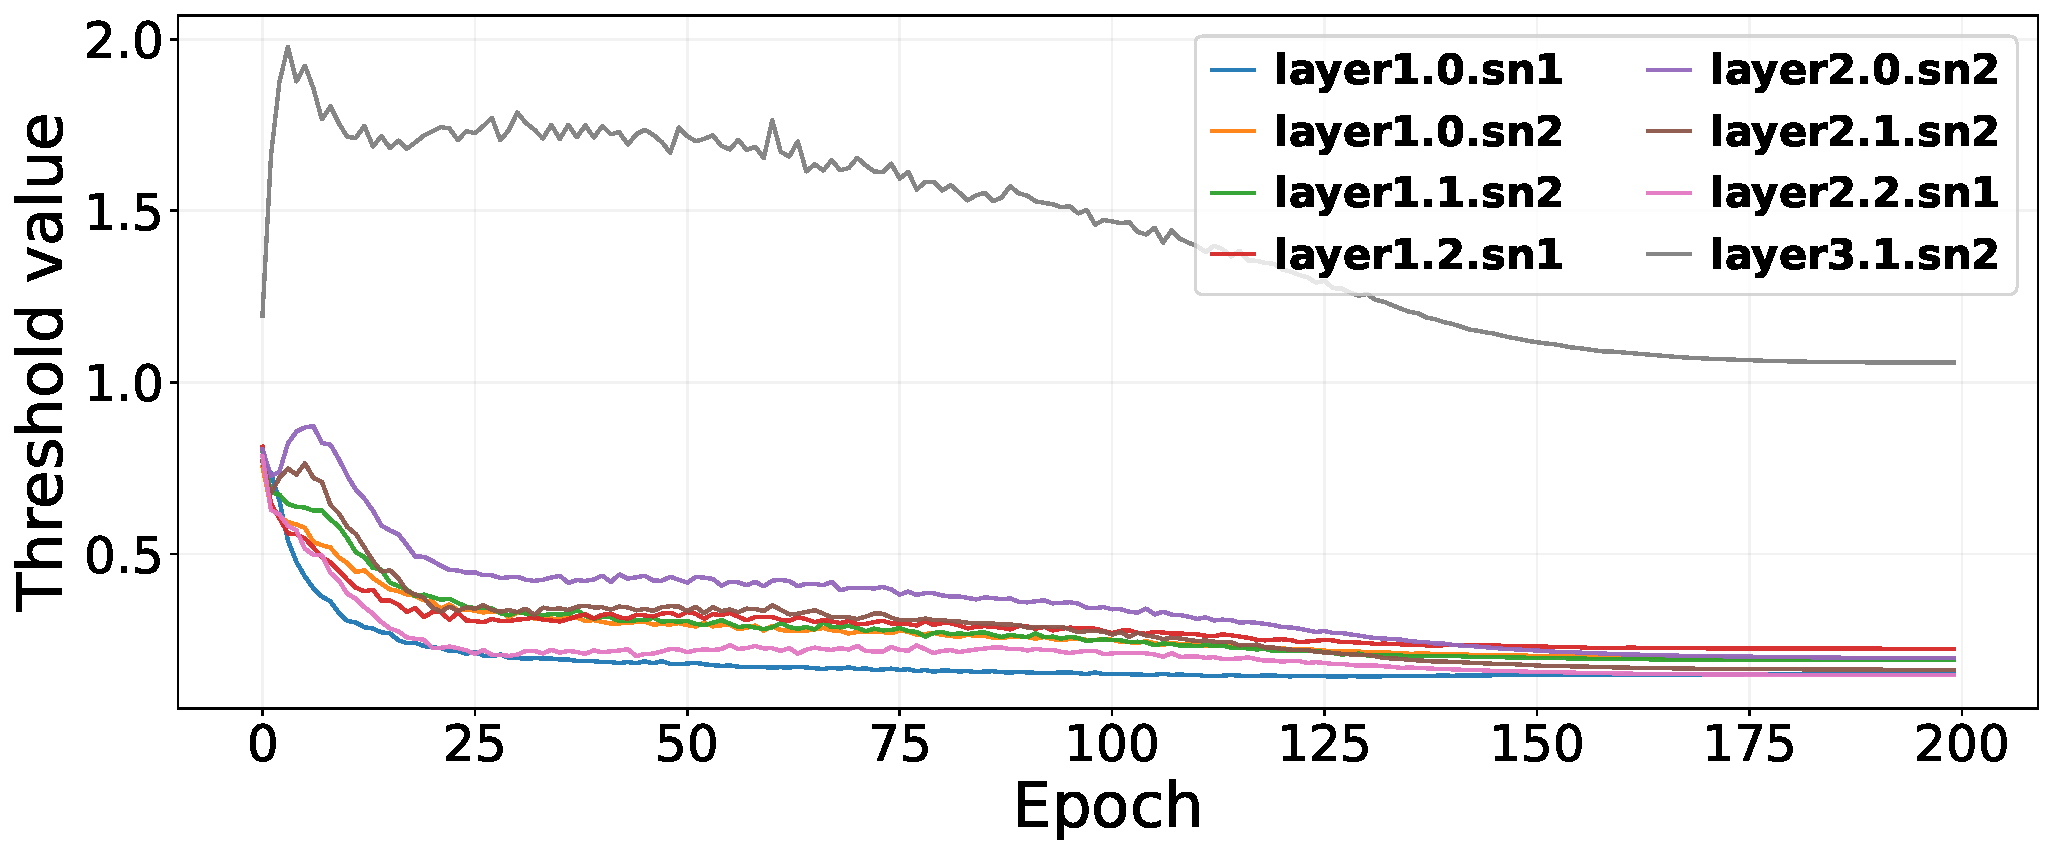
\includegraphics[width=\linewidth]{fig/threshold_training_cifar100.pdf}
    \caption{ResNet-19 on CIFAR100}
  \end{subfigure}
  \hfill
  \begin{subfigure}[b]{0.99\linewidth}
    \centering
    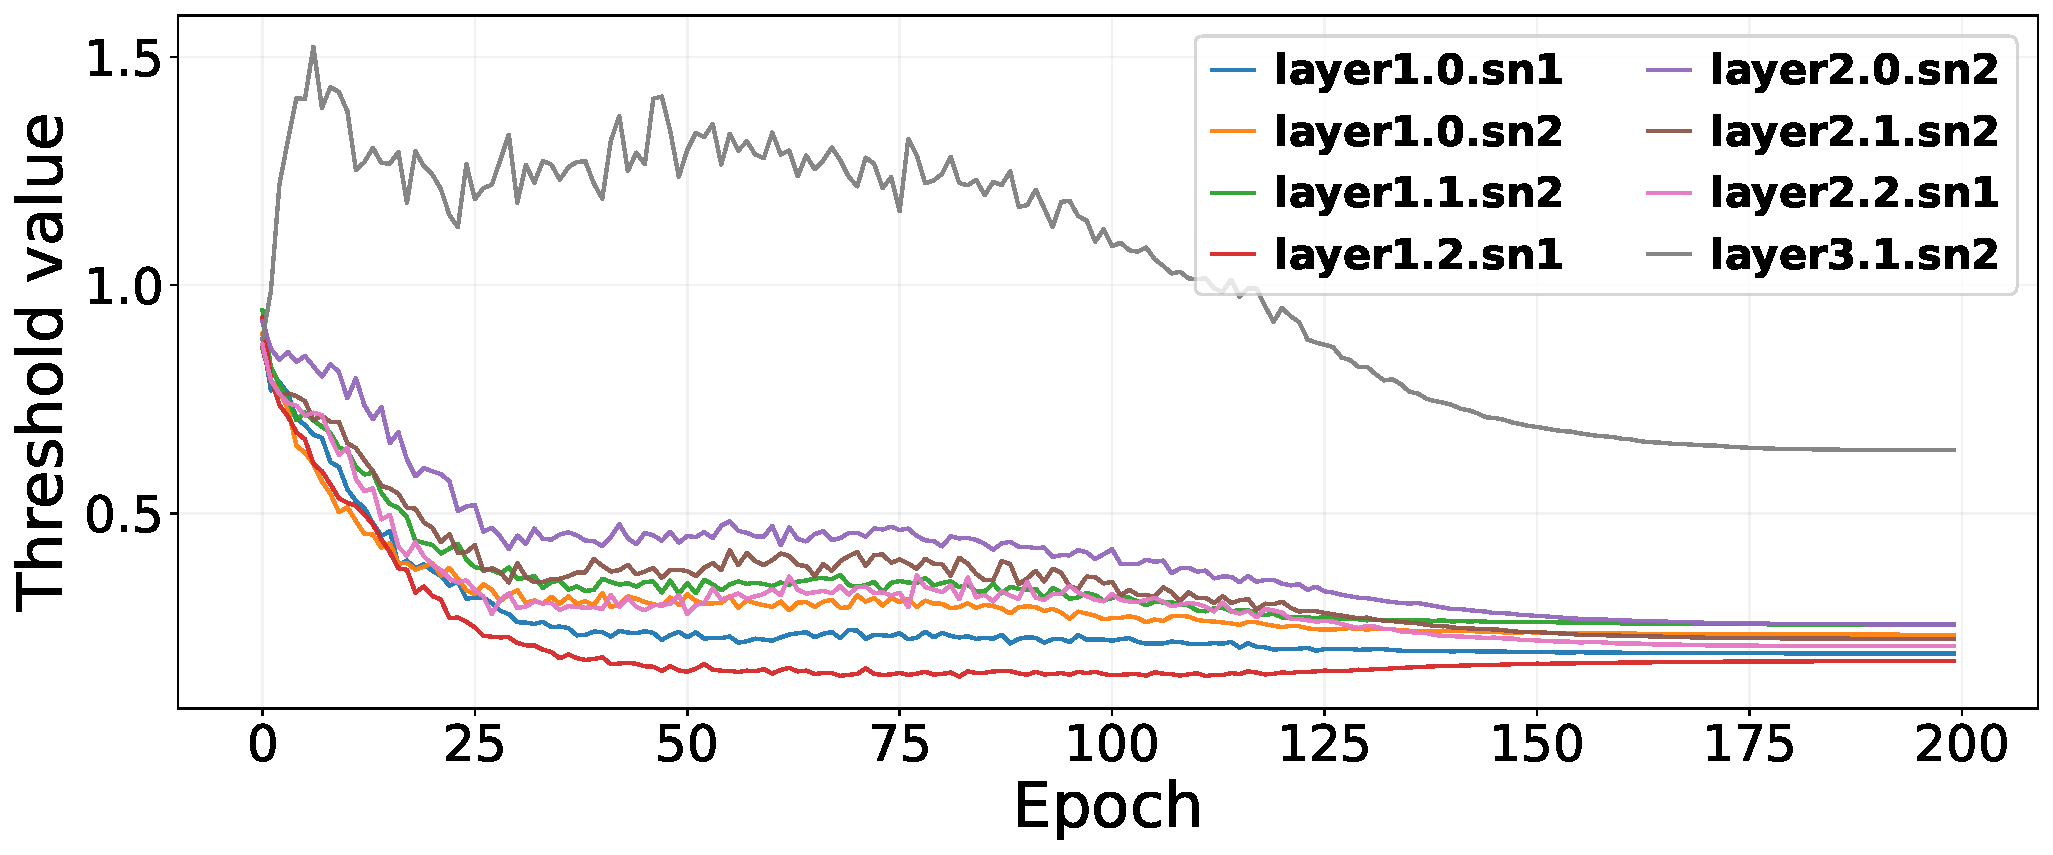
\includegraphics[width=\linewidth]{fig/threshold_training_dvscifar10.pdf}
    \caption{ResNet-19 on DVS-CIFAR10}
  \end{subfigure}
  \hfill
  \begin{subfigure}[b]{0.99\linewidth}
    \centering
    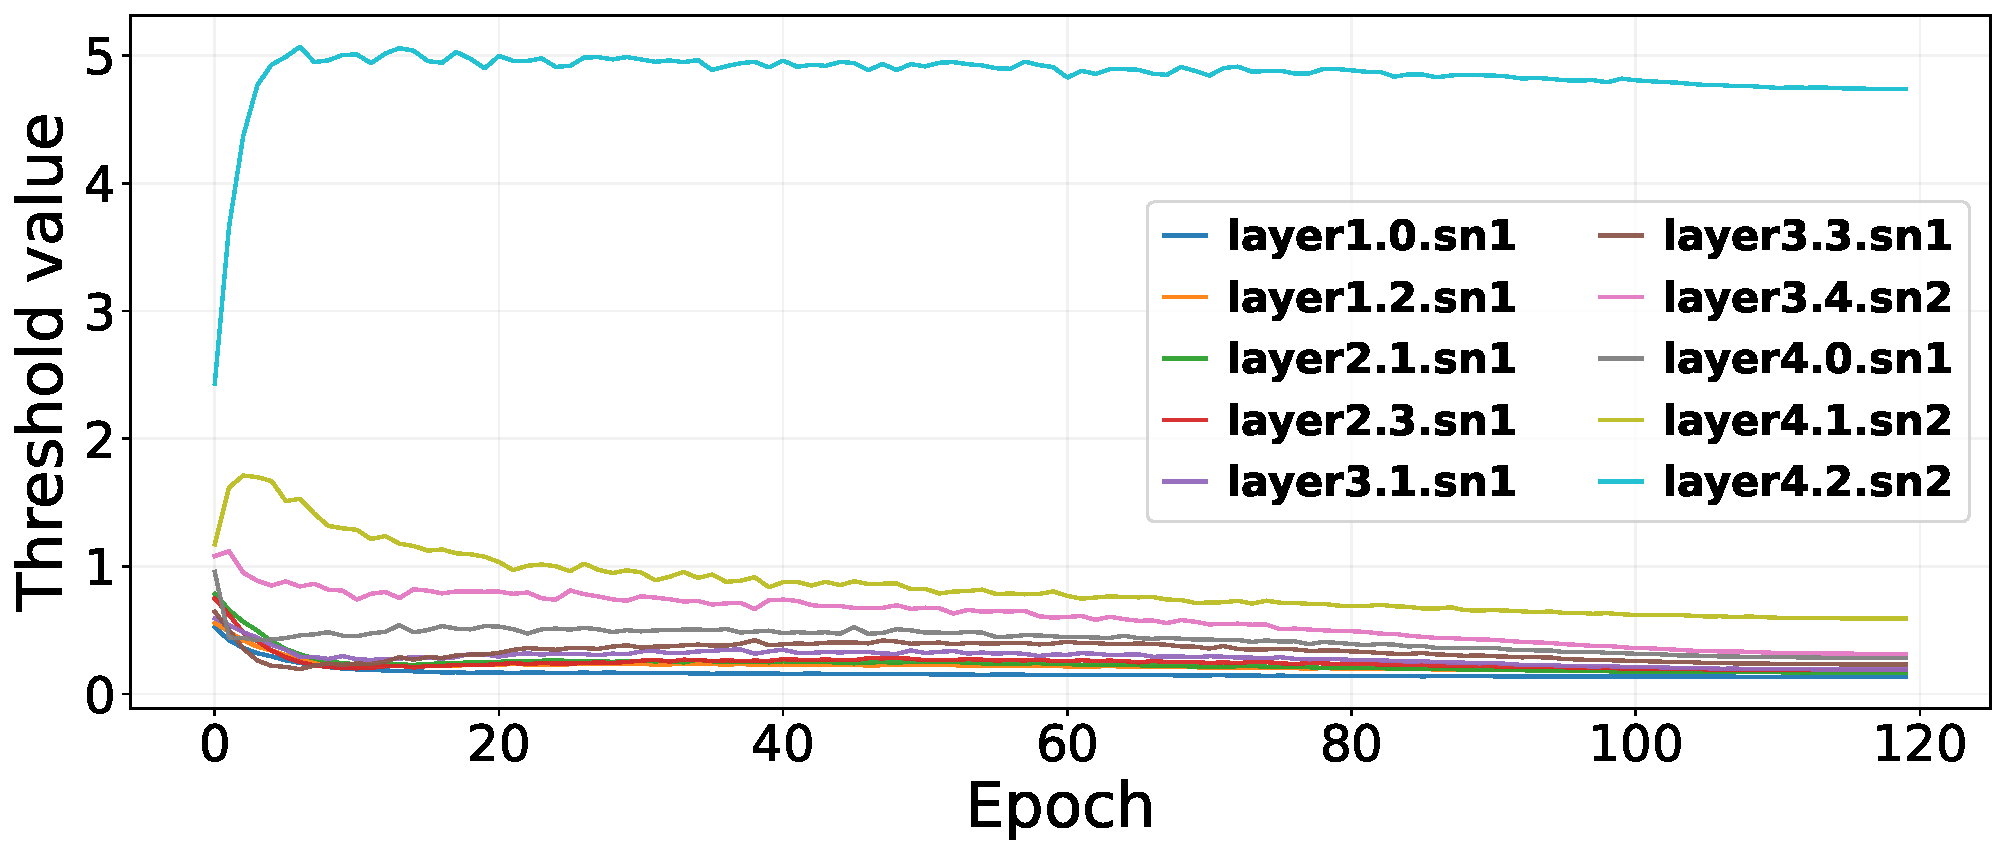
\includegraphics[width=\linewidth]{fig/threshold_training_imagenet.pdf}
    \caption{ResNet-34 on ImageNet}
  \end{subfigure}
  \caption{\textbf{Trajectories of trainable $V_{\text{thr}}$ during training.} 
  Early layers tend to settle at lower thresholds, while late/deep layers increase toward larger thresholds.}
  \label{fig:vthr_dynamics}
\end{figure}

\paragraph{Implications:}

\begin{itemize}
\item \cref{tab:metrics_ref,tab:metrics_low,tab:metrics_high} explain \emph{why} TrSG is superior: it maintains moderate magnitude (AbsStr), healthy selectivity (RatioAG), and low update variance (GradCV), avoiding flood/starvation and explosion/vanishing. 

\item The threshold trajectories in \cref{fig:vthr_dynamics} show that real trainings \emph{do} visit the very regimes that break AS-SG/RS-SG, so threshold-robustness is not a corner case but a practical necessity. 

\item \textbf{Even when $V_{\text{thr}}$ and $\tau$ are not trained}, TrSG remains the best choice across thresholds (\cref{tab:no_training_results}); using TrSG is strictly beneficial, with no downside in practice.
\end{itemize}

\subsection{Ablation on Advanced Architecture}
\label{subsec:ablation_large_transformer}

\begin{table}[h]
\centering
\small
\begin{tabular}{lc}
\toprule
\textbf{Method} & \textbf{Top-1 (\%)} \\
\midrule
QKFormer (HST-10-384) & 78.80 \\
\quad + AS-SG         & 77.09 \\
\quad + RS-SG         & 78.70 \\
\quad \textbf{+ TrSG} & \textbf{79.90} \\
\bottomrule
\end{tabular}
\caption{Ablation on surrogate gradient choice for QKFormer (HST-10-384) on ImageNet at 4 timesteps. 
All runs follow the official training recipe; only the SG variant differs. 
MP-Init is enabled in all cases.}
\label{tab:qkformer_ablation}
\end{table}

We ablate the surrogate gradient formulation on a large-scale Transformer SNN, QKFormer~\cite{zhou:2024_2}, using the official training protocol while keeping all settings fixed and changing only the SG type. With MP-Init enabled across the board, \textbf{TrSG} is the only variant that reliably improves over the baseline ($+1.10$ \%pt), whereas \textbf{AS-SG} underperforms ($-1.71$ \%pt) and \textbf{RS-SG} essentially matches or slightly underperforms ($-0.10$ \%pt). 

These results demonstrate that even on advanced Transformer-based SNNs, TrSG provides consistent benefits. More importantly, they show that using conventional SGs not only fails to deliver improvements but can actually degrade performance, underscoring TrSG as the superior and safer choice for training modern large-scale SNN architectures.


\begin{figure}[t]
  \centering
  \begin{subfigure}{0.99\linewidth}
    \centering
    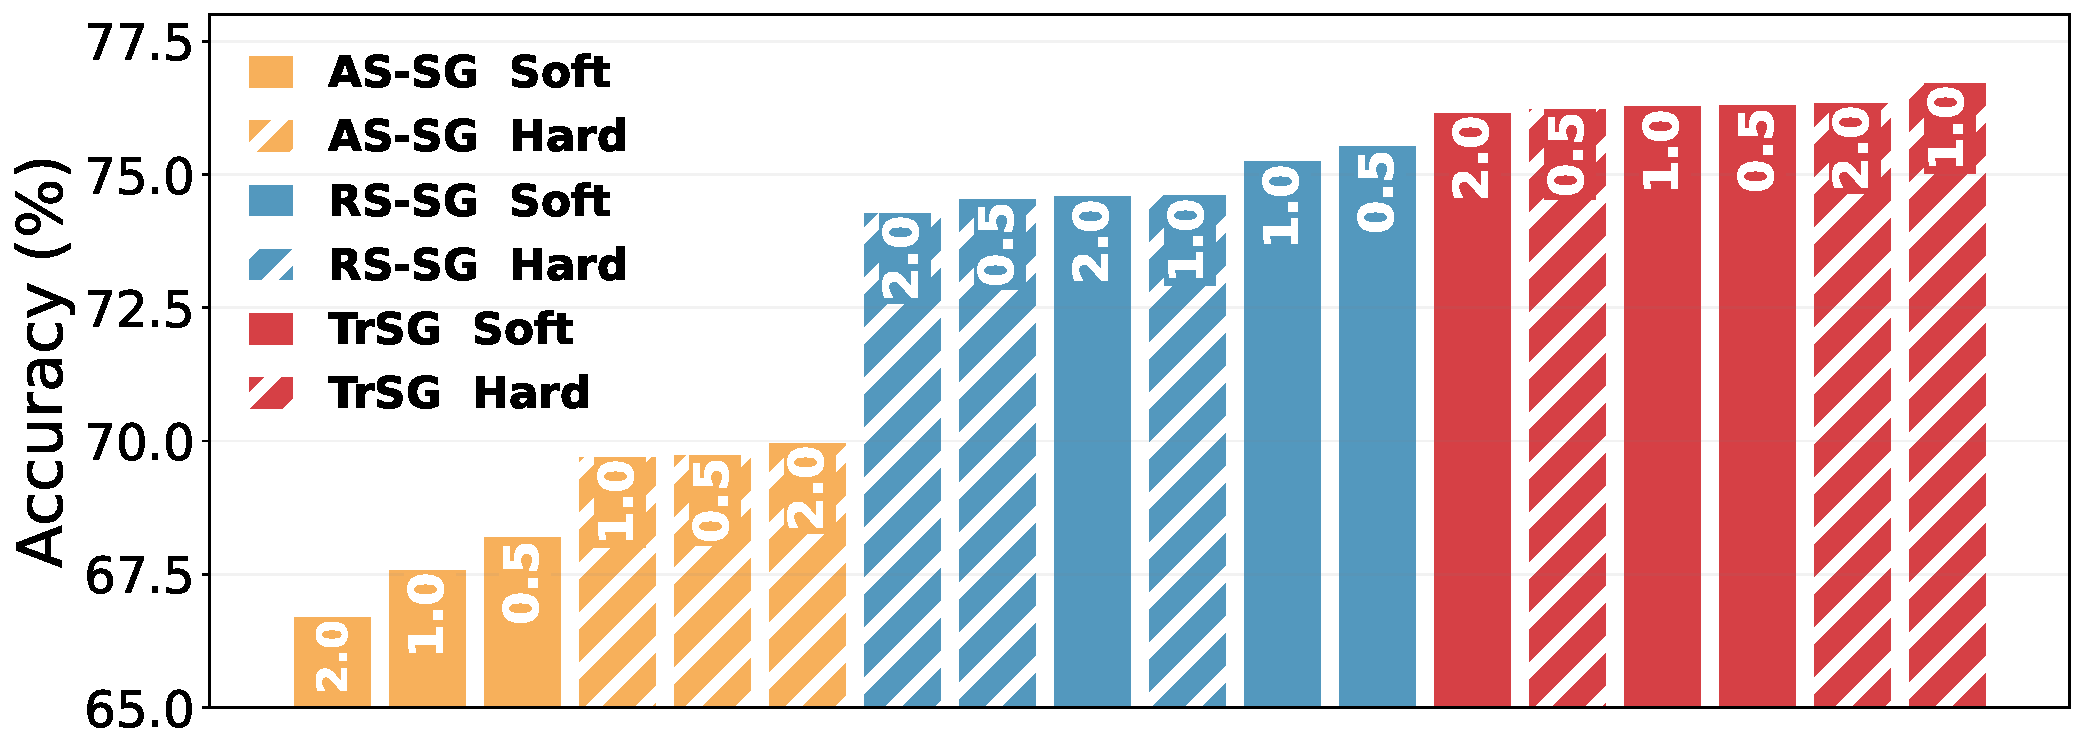
\includegraphics[width=0.99\linewidth]{fig/acc_different_thr_atan.pdf}
    \caption{Arctan: init \(\tau=2.0,V_{\text{thr}}\in\{0.5,1.0,2.0\}\)}
  \end{subfigure}
  \begin{subfigure}{0.99\linewidth}
    \centering
    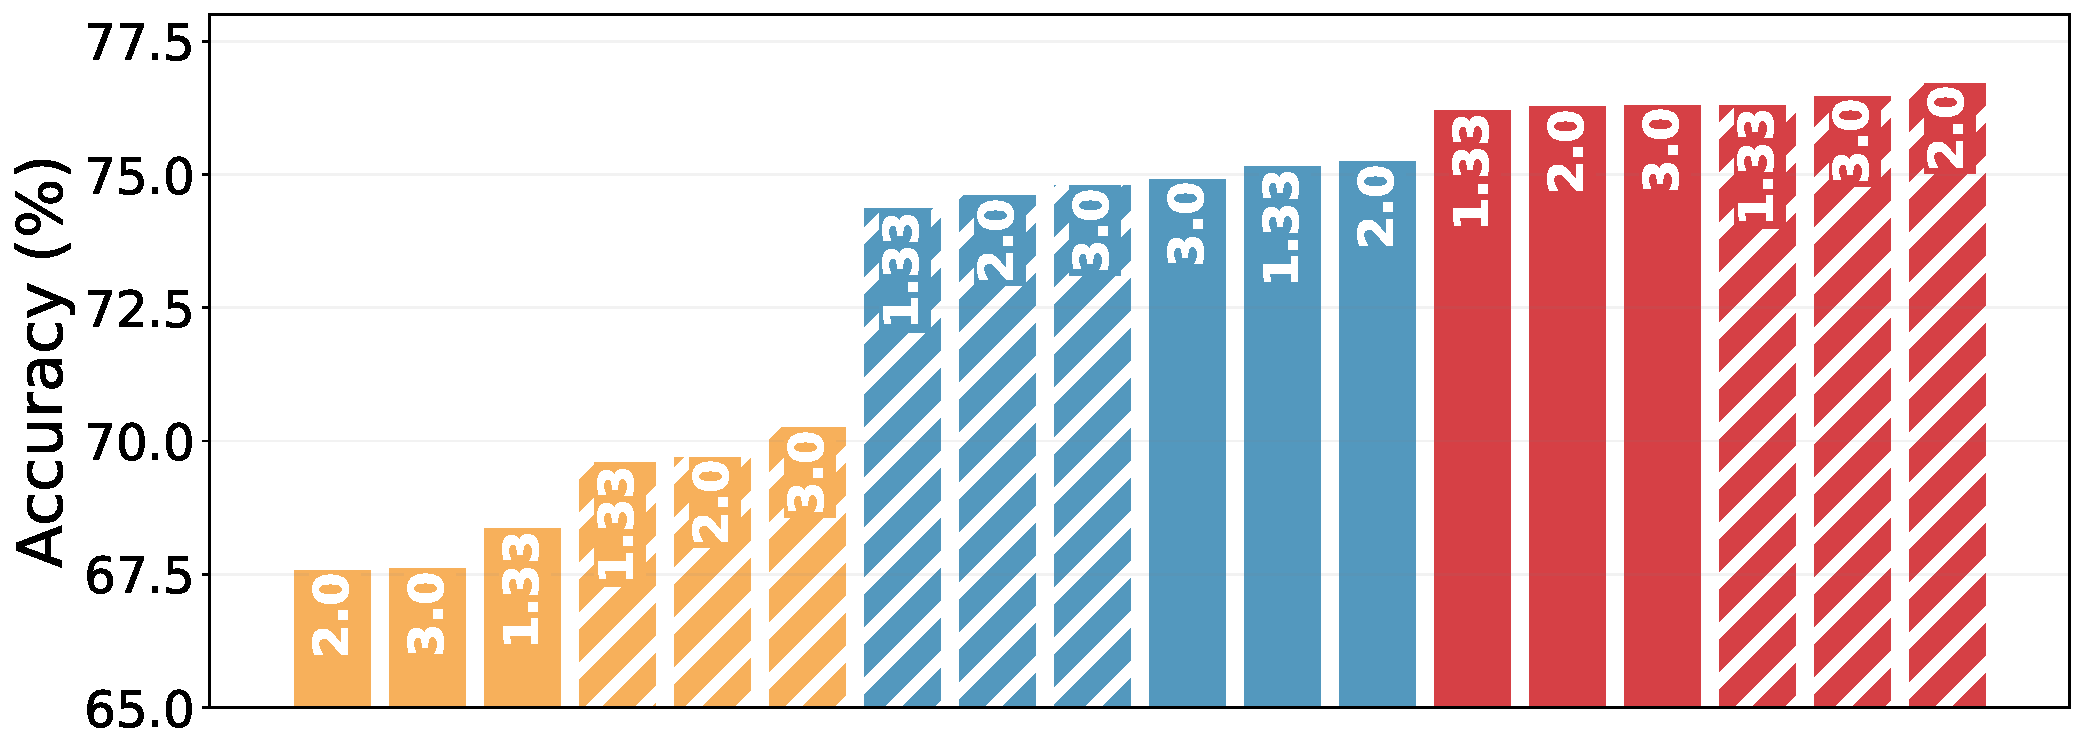
\includegraphics[width=0.99\linewidth]{fig/acc_different_tau_atan.pdf}
    \caption{Arctan: init \(V_{\text{thr}}=1.0,\tau\in\{1.33,2.0,3.0\}\)}
  \end{subfigure}
  \begin{subfigure}{0.99\linewidth}
    \centering
    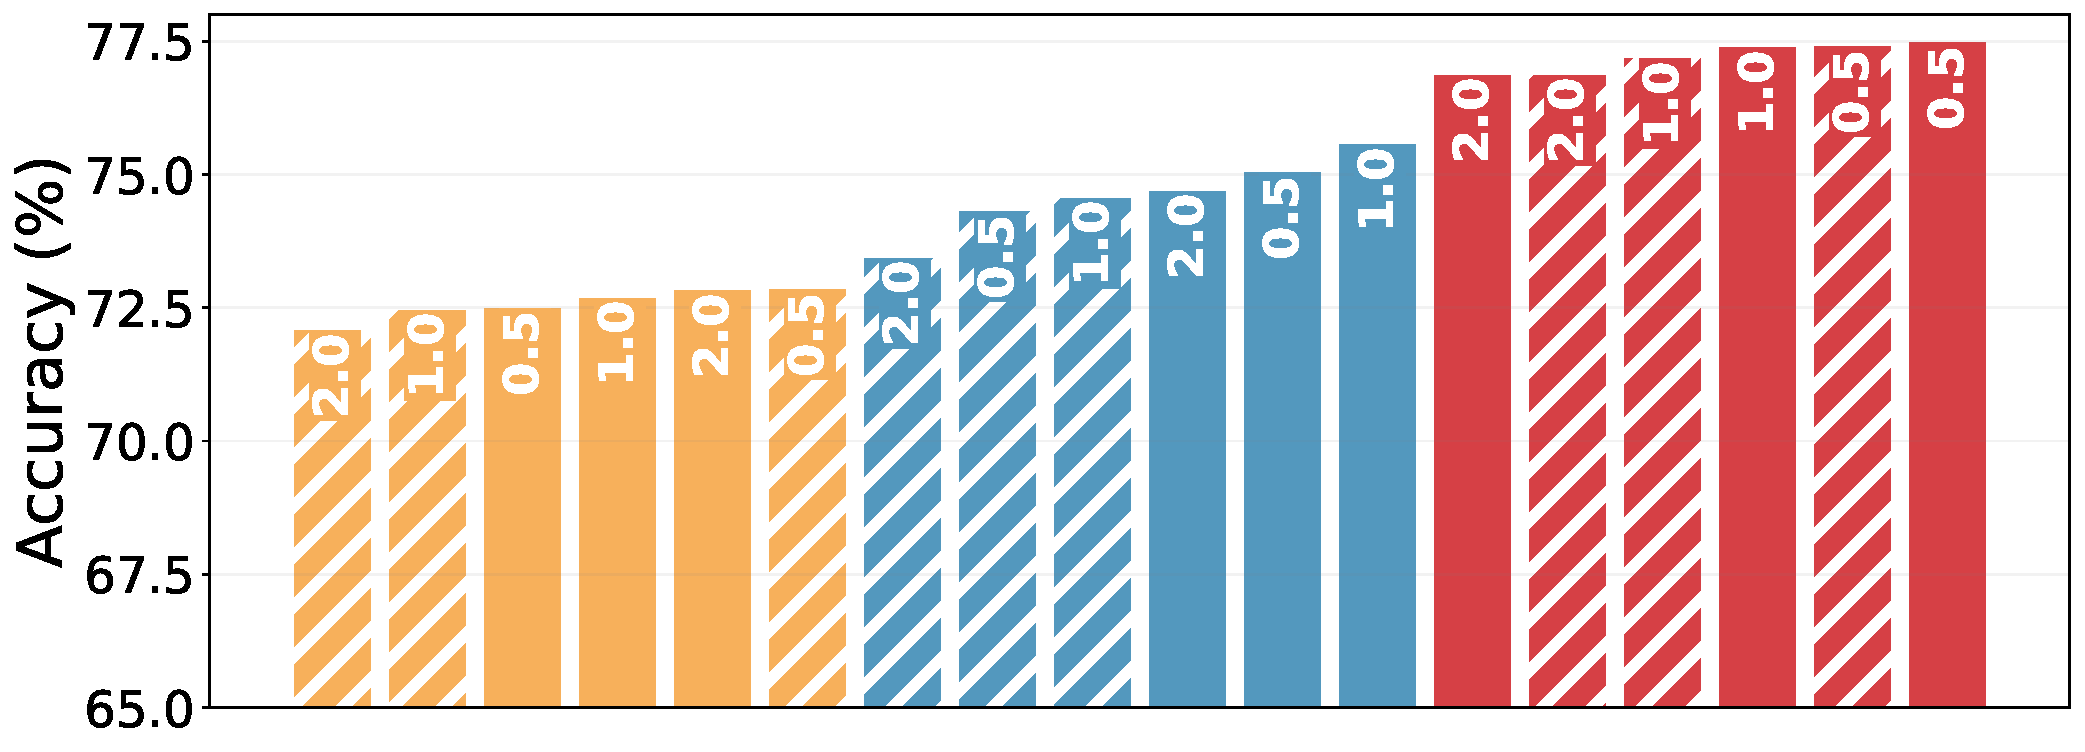
\includegraphics[width=0.99\linewidth]{fig/acc_different_thr_sigmoid.pdf}
    \caption{Sigmoid: init \(\tau=2.0,V_{\text{thr}}\in\{0.5,1.0,2.0\}\)}
  \end{subfigure}
  \begin{subfigure}{0.99\linewidth}
    \centering
    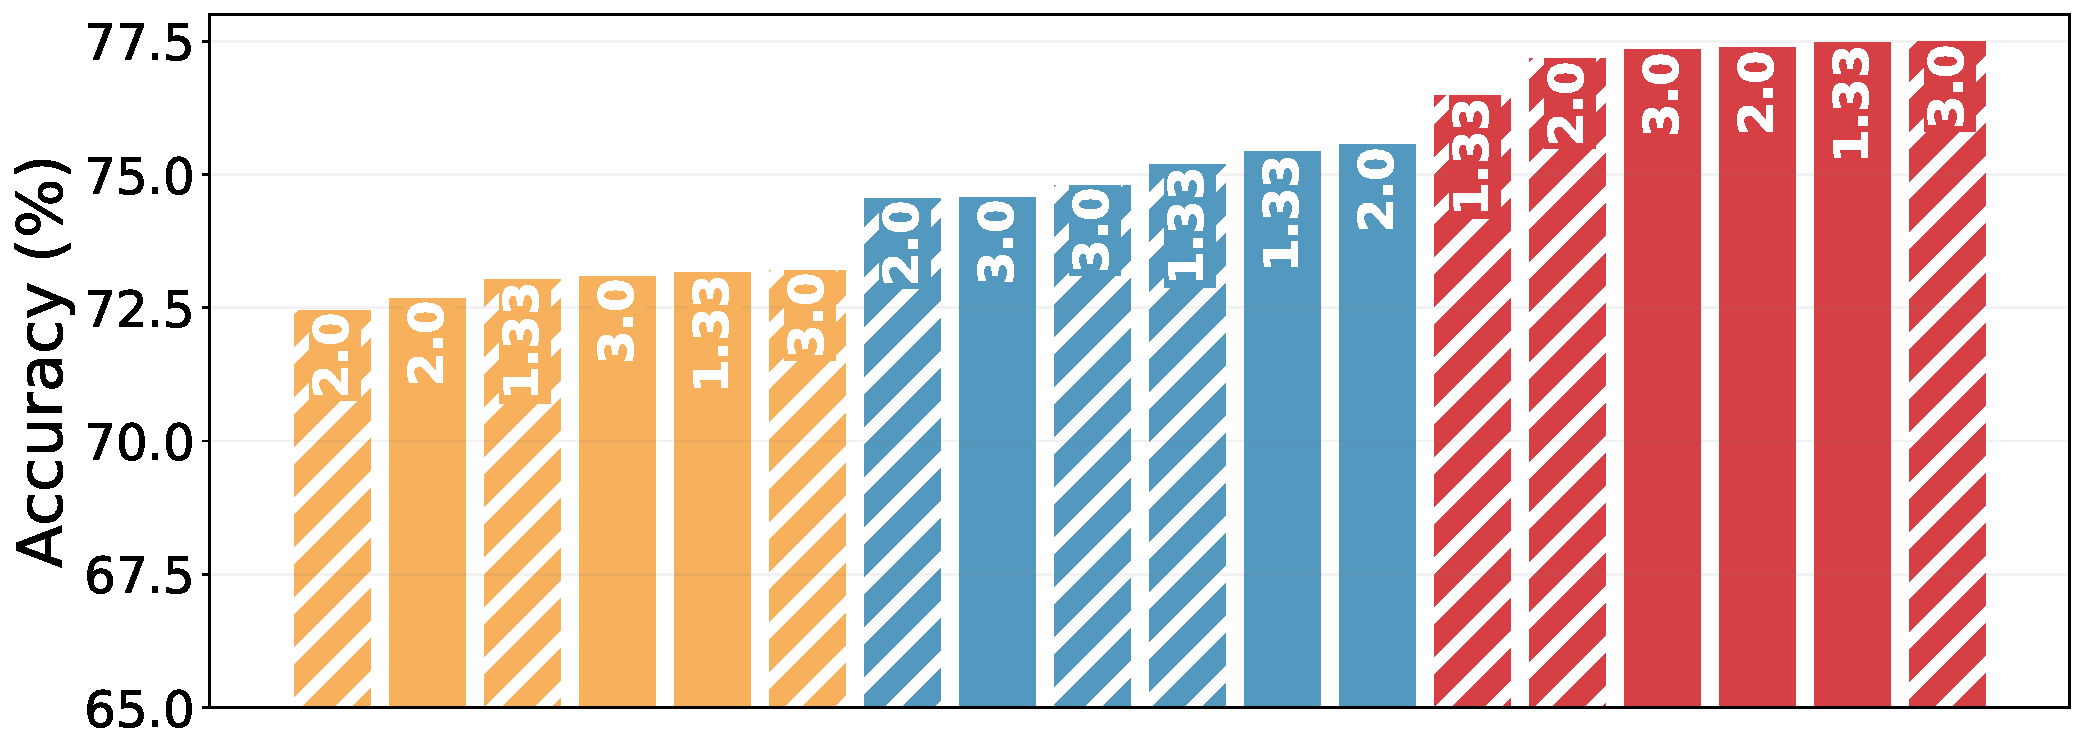
\includegraphics[width=0.99\linewidth]{fig/acc_different_tau_sigmoid.pdf}
    \caption{Sigmoid: init \(V_{\text{thr}}=1.0,\tau\in\{1.33,2.0,3.0\}\)}
  \end{subfigure}
  \caption{\textbf{Accuracy under different initial values of \(\tau\) and \(V_{\text{thr}}\) when learning both parameters, using the \emph{Arctan} and \emph{Sigmoid} surrogate function.} \textbf{(Top)}: The results using Arctan surrogate function. \textbf{(Bottom)}: The results using Sigmoid surrogate function. We compare AS-SG, RS-SG, and \textbf{TrSG} on a ResNet-19 (CIFAR100, 4 timesteps), evaluating both soft- and hard-reset LIF neurons.}
  \label{fig:acc_different_atan}
\end{figure}

\subsection{Validation on More Surrogate Functions}
\label{subsec:validation_of_atan}

In \cref{sec:second_method}, we introduced \textbf{TrSG (Threshold-robust Surrogate Gradient)} using a Rectangular-shaped surrogate as our primary example. In \cref{subsec:analysis_of_ta}, we extended experiments to include a Triangular-shaped surrogate. Here, we further demonstrate TrSG’s generality by evaluating it with an Arctan-based~\cite{fang:2021} and Sigmoid-based~\cite{wu:2018} surrogate functions.

\paragraph{Arctan Surrogate Function}
For an Arctan-based neuron, the derivative of the surrogate firing function is expressed as:
\[
    \frac{\partial f_{sr}(x)}{\partial x}
    \;=\; 
    \frac{\gamma}{\,2 \Bigl(1 + \bigl(\tfrac{\pi}{2}\,\gamma\,x\bigr)^{2}\Bigr)\!}.
\]

\paragraph{Sigmoid Surrogate Function}
For a Sigmoid-based neuron, the derivative of the surrogate firing function is expressed as:
\[
    \frac{\partial f_{sr}(x)}{\partial x}
    \;=\; 
    \frac{1}{\gamma}\frac{e^{\frac{x}{\gamma}}}{(1+e^{\frac{x}{\gamma}})^2}.
\]

where \(\gamma\) is the steepness parameter. Similar to our earlier analyses, we compare three SG methods (AS-SG, RS-SG, and \textbf{TrSG}) under both soft and hard reset neuron models.

\cref{fig:acc_different_atan} shows that \textbf{TrSG} consistently outperforms the conventional \textbf{absolute-scale} (AS-SG) and \textbf{relative-scale} (RS-SG) approaches, regardless of the initial threshold or time constant. This robust behavior parallels our findings in \cref{subsec:analysis_of_ta} for Rectangular and Triangular surrogates. TrSG maintains reliable performance across a wide range of initial conditions, emphasizing its capacity to provide stable gradient flow even for varied neuron parameters.

\subsection{Surrogate Gradient Through \texorpdfstring{\(V_{\text{thr}}^l\) and \(\tau^l\)}{}}
\label{subsec:grad_vthr_tau}

In the main text, our analysis of threshold-related instabilities centered primarily on 
\[
\frac{\partial S^l[t]}{\partial M^l[t]},
\]
i.e., how the spike output changes with respect to the membrane potential. 
However, similar issues arise when considering partial derivatives w.r.t.\ \(V_{\text{thr}}^l\) and \(\tau^l\). 
Below, we illustrate how AS-SG and RS-SG can each fail to provide stable gradients in these pathways and then show how \textbf{TrSG} maintains a consistent and well-scaled gradient flow.

\paragraph{1. Gradient w.r.t.\ \texorpdfstring{\(V_{\text{thr}}^l\)}{Vthr}.}
Recall from \cref{eq:lif_discrete_firing} that
\(
S^l[t] = \mathcal{H}(\,M^l[t] - V_{\text{thr}}^l\,)
\).
When approximating \(\mathcal{H}\) by a differentiable surrogate \(f_{sr}\), existing methods define the argument \(x\) in either \textbf{absolute-scale} or \textbf{relative-scale} form:

\begin{itemize}
    \item \textbf{AS-SG (Absolute-Scale).}  
    \(
    x = M^l[t] - V_{\text{thr}}^l.
    \)
    Then, 
    \[
    \frac{\partial S^l[t]}{\partial V_{\text{thr}}^l}
    \;=\;
    f_{sr}'(x)\,\times \Bigl(\tfrac{\partial M^l[t]}{\partial V_{\text{thr}}^l} - 1\Bigr),
    \]
    whose update does not adapt its magnitude to \(V_{\text{thr}}^l\). Consequently, if \(|V_{\text{thr}}^l|\) becomes very large or very small, the gradient can vanish or dominate excessively.

    \item \textbf{RS-SG (Relative-Scale).}  
    \(
    x = \tfrac{M^l[t]}{V_{\text{thr}}^l} - 1.
    \)
    By the chain rule,
    \[
    \frac{\partial S^l[t]}{\partial V_{\text{thr}}^l}
    \;\approx\;
    f_{sr}'\!\bigl(\tfrac{M^l[t]}{V_{\text{thr}}^l}-1\bigr)\,\times\,\tfrac{\partial}{\partial V_{\text{thr}}^l}\!\Bigl(\tfrac{M^l[t]}{V_{\text{thr}}^l}-1\Bigr),
    \]
    which can introduce factors proportional to \(\tfrac{1}{V_{\text{thr}}^l}\). If \(V_{\text{thr}}^l\) is tiny, the gradient risk is explosion; if \(V_{\text{thr}}^l\) is huge, updates can vanish.
\end{itemize}

\textbf{TrSG} circumvents both extremes by using a relative-scale definition for \(x\) and multiplying \(V_{\text{thr}}^l\) forward during training:
\[
O^l[t] \;=\; V_{\text{thr}}^l\,S^l[t].
\]
As discussed in the main text, this multiplication cancels out the problematic \(\tfrac{1}{V_{\text{thr}}^l}\) factor during backpropagation, keeping gradients w.r.t.\ \(V_{\text{thr}}^l\) stable throughout training.

\paragraph{2. Gradient w.r.t.\ \texorpdfstring{\(\tau^l\)}{tau}.}
Next, consider the discrete LIF update from \cref{eq:lif_discrete_potential}:
\(
M^l[t]
\;=\;
\Bigl(1 - \tfrac{1}{\tau^l}\Bigr)\,U^l[t-1]
\;+\;
\tfrac{1}{\tau^l}\,I_{\text{in}}^l[t]
\).
Since \(\tau^l\) appears in denominators, it affects \(S^l[t]\) indirectly via \(M^l[t]\). Hence,
\[
\frac{\partial S^l[t]}{\partial \tau^l}
\;=\;
\frac{\partial S^l[t]}{\partial M^l[t]}
\;\times\;
\frac{\partial M^l[t]}{\partial \tau^l}.
\]
If \(\tfrac{\partial S^l[t]}{\partial M^l[t]}\) is not well-scaled (as in standard AS-SG or RS-SG), the \(\tfrac{\partial S^l[t]}{\partial \tau^l}\) may yield exploding or vanishing updates. 
\textbf{TrSG}, by ensuring a stable gradient path for \(\tfrac{\partial S^l[t]}{\partial M^l[t]}\), similarly prevents instability when learning \(\tau^l\).

In conclusion, TrSG’s threshold-multiplication mechanism and relative-scale formulation ensure that gradients remain appropriately scaled not only w.r.t.\ \(M^l[t]\) but also along the \(V_{\text{thr}}^l\) and \(\tau^l\) pathways. This provides a broad foundation for stable, end-to-end training of spiking neurons, even when multiple internal parameters are learnable.


\section{Additional Experimental Results}
\label{sec:suppl_additional_exp}

\begin{figure}[h]
  \centering
  \begin{subfigure}{0.99\linewidth}
    \centering
    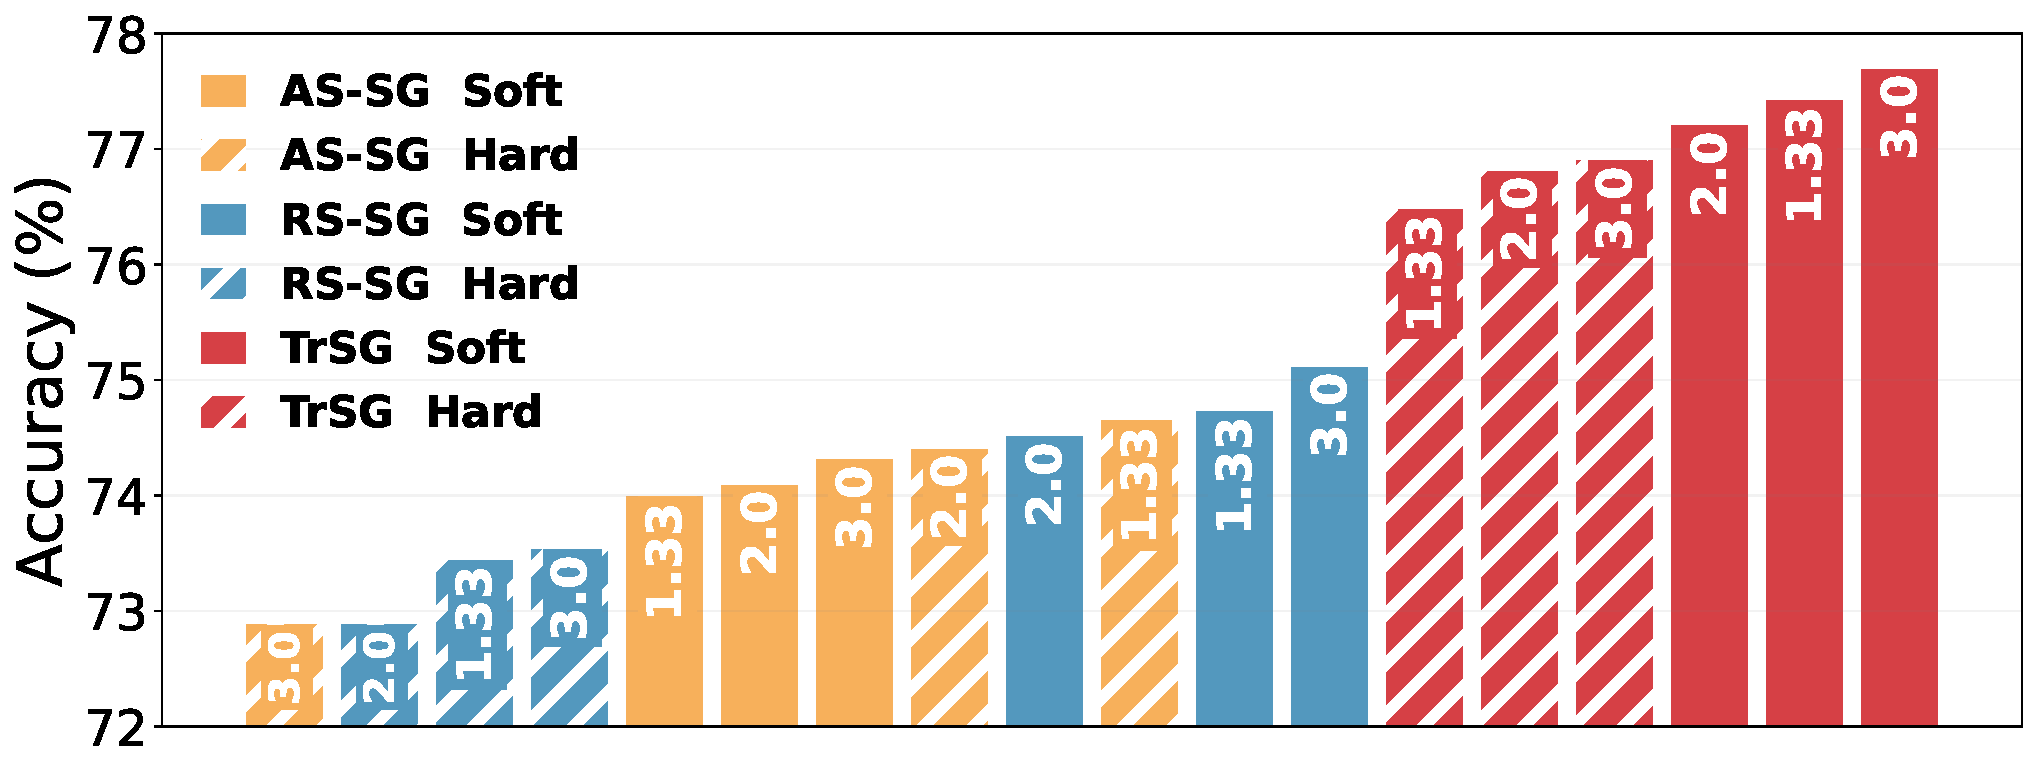
\includegraphics[width=0.99\linewidth]{fig/acc_different_tau_rect.pdf}
    \caption{Rectangular-shaped Surrogate Gradient}
    \label{fig:acc_different_tau_rect}
  \end{subfigure}
  \vspace{0.4em}
  \begin{subfigure}{0.99\linewidth}
    \centering
    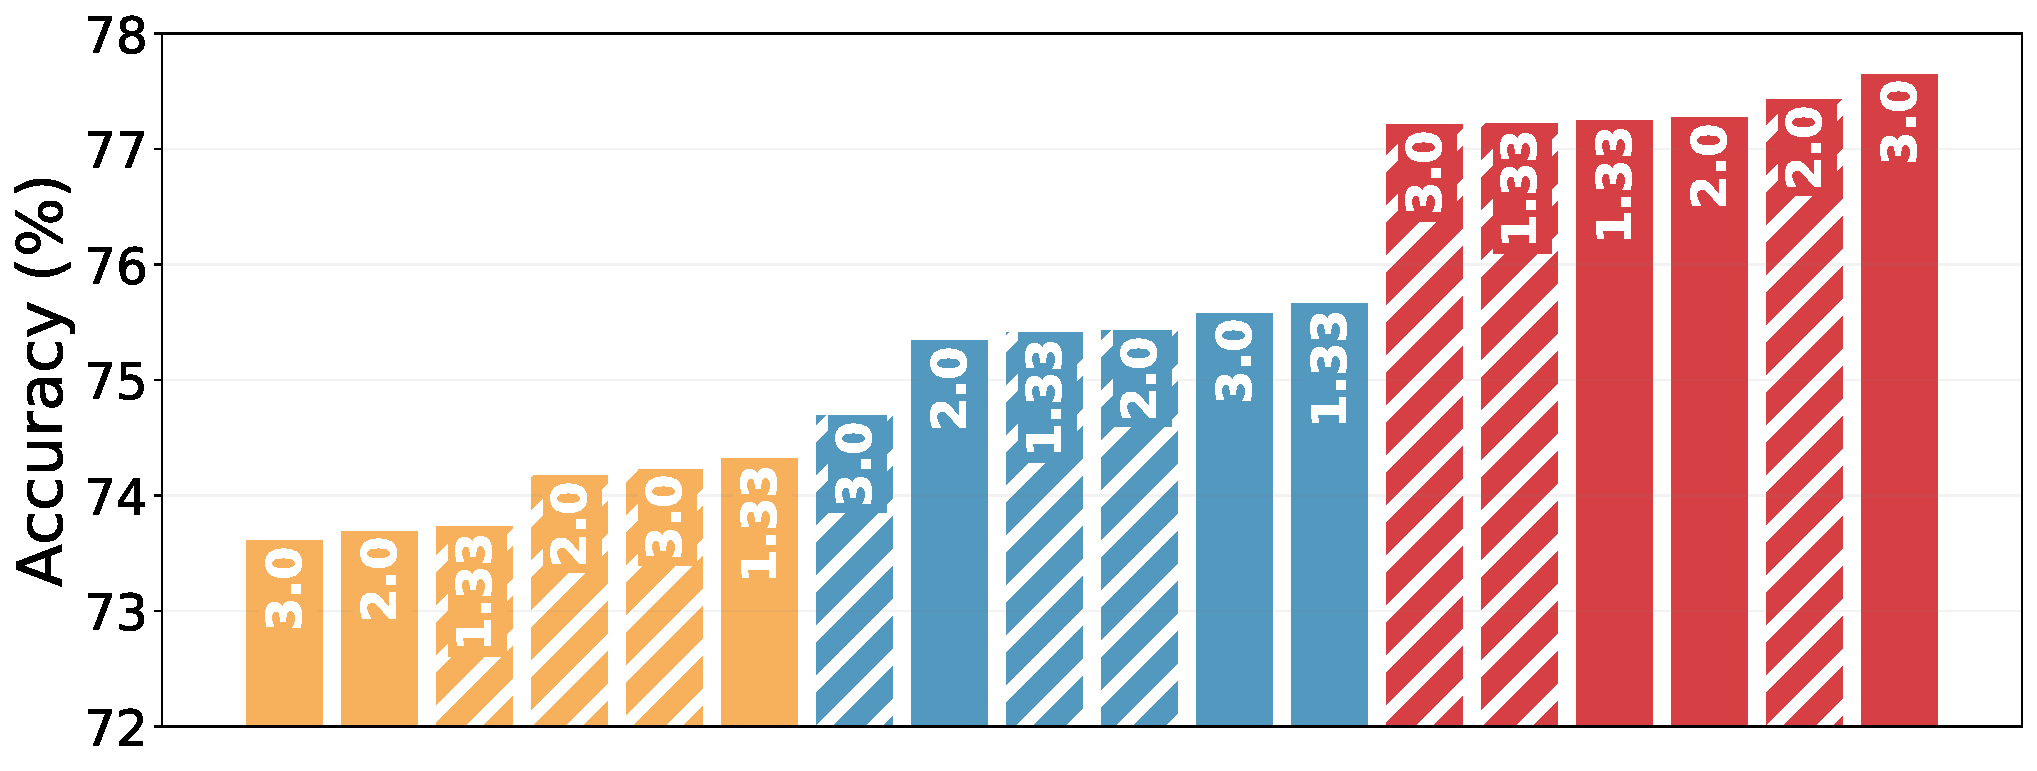
\includegraphics[width=0.99\linewidth]{fig/acc_different_tau_tri.pdf}
    \caption{Triangular-shaped Surrogate Gradient}
    \label{fig:acc_different_tau_tri}
  \end{subfigure}
  \caption{
    \textbf{Accuracy results with different initial \(\tau\) values with initial \(V_{\text{thr}} = 1.0\).} We compare three SG types \textbf{(i) AdSG} \textbf{(i) RdSG} \textbf{(i) TrSG} under two shapes
    \textbf{(a)}~Rectangular and \textbf{(b)}~Triangular, each with both soft and hard resets. We vary initial \(\tau \in \{1.33,2.0,3.0\}\), indicated in the bars, and train ResNet-19 on CIFAR100 using 4 timesteps.
  }
  \label{fig:acc_different_tau_rect_tri}
\end{figure}

\subsection{Varying Initial \texorpdfstring{\(\tau\)}{} with a Fixed Initial \texorpdfstring{\(V_{\text{thr}}\)}{}}
\label{subsec:tau_var_supp}


To further complement the experiments in \cref{subsec:analysis_of_ta}, 
we conduct additional tests where we fix the initial threshold \(\,V_{\text{thr}}=1.0\) and instead vary the initial time constant \(\,\tau \in \{1.33,\,2.0,\,3.0\}\).  In \cref{fig:acc_different_tau_rect_tri}, the top panel 
(\cref{fig:acc_different_tau_rect}) reports accuracy under the Rectangular-shaped surrogate gradient, while the bottom panel (\cref{fig:acc_different_tau_tri}) corresponds to the Triangular-shaped surrogate. Each panel compares three SG types (AdSG, RdSG, and TrSG) and two reset modes (soft vs.\ hard). 

Our proposed \textbf{TrSG} consistently outperforms AS-SG and RS-SG across all initial \(\tau\) values. TrSG maintains high accuracy in every setting, demonstrating its robust learning dynamics and further validating the overall trend observed in \cref{subsec:analysis_of_ta}.

\begin{table}[t]
    \centering
    \begin{tabular}{ccc}
        \toprule
        \(\tau\) & \(V_{\text{thr}}\) & Accuracy (\%) \\
        \midrule
        \ding{55} & \ding{55} & 75.56 \\
        \ding{51} & \ding{55} & 74.61 \\
        \ding{55} & \ding{51} & 76.98 \\
        \ding{51} & \ding{51} & 77.22 \\
        \bottomrule
    \end{tabular}
    \caption{Ablation study of trainable parameters on ResNet-19 trained on CIFAR-100 with a timestep of 4. The initial (or fixed) values for \(V_{\text{thr}}\) and \(\tau\) are set to 1.0 and 2.0, respectively. \(\checkmark\) indicates trainable, while \(\text{\texttimes}\) means not trainable.}
    \label{tab:ablation_study}
\end{table}

\subsection{Impact of Trainable Parameters on Accuracy}

To analyze the impact of training the threshold potential \(V_{\text{thr}}\) and the time decay constant \(\tau\), we conduct an ablation study. The results are summarized in \cref{tab:ablation_study}.

From \cref{tab:ablation_study}, we observe that training only \(\tau\) results in a slight degradation in accuracy compared to fixed parameters. In contrast, training \(V_{\text{thr}}\) alone leads to a noticeable improvement in accuracy. Moreover, training \(\tau\) alongside \(V_{\text{thr}}\) yields the best results, with a final accuracy of 77.22\%. 

This indicates that while training \(\tau\) alone may not be beneficial, its effect becomes synergistic when combined with \(V_{\text{thr}}\) training. By allowing both parameters to be learned, the model can dynamically adjust them to achieve a balance between convergence speed and network stability, thereby enhancing performance.

\begin{figure}[h]
  \centering
  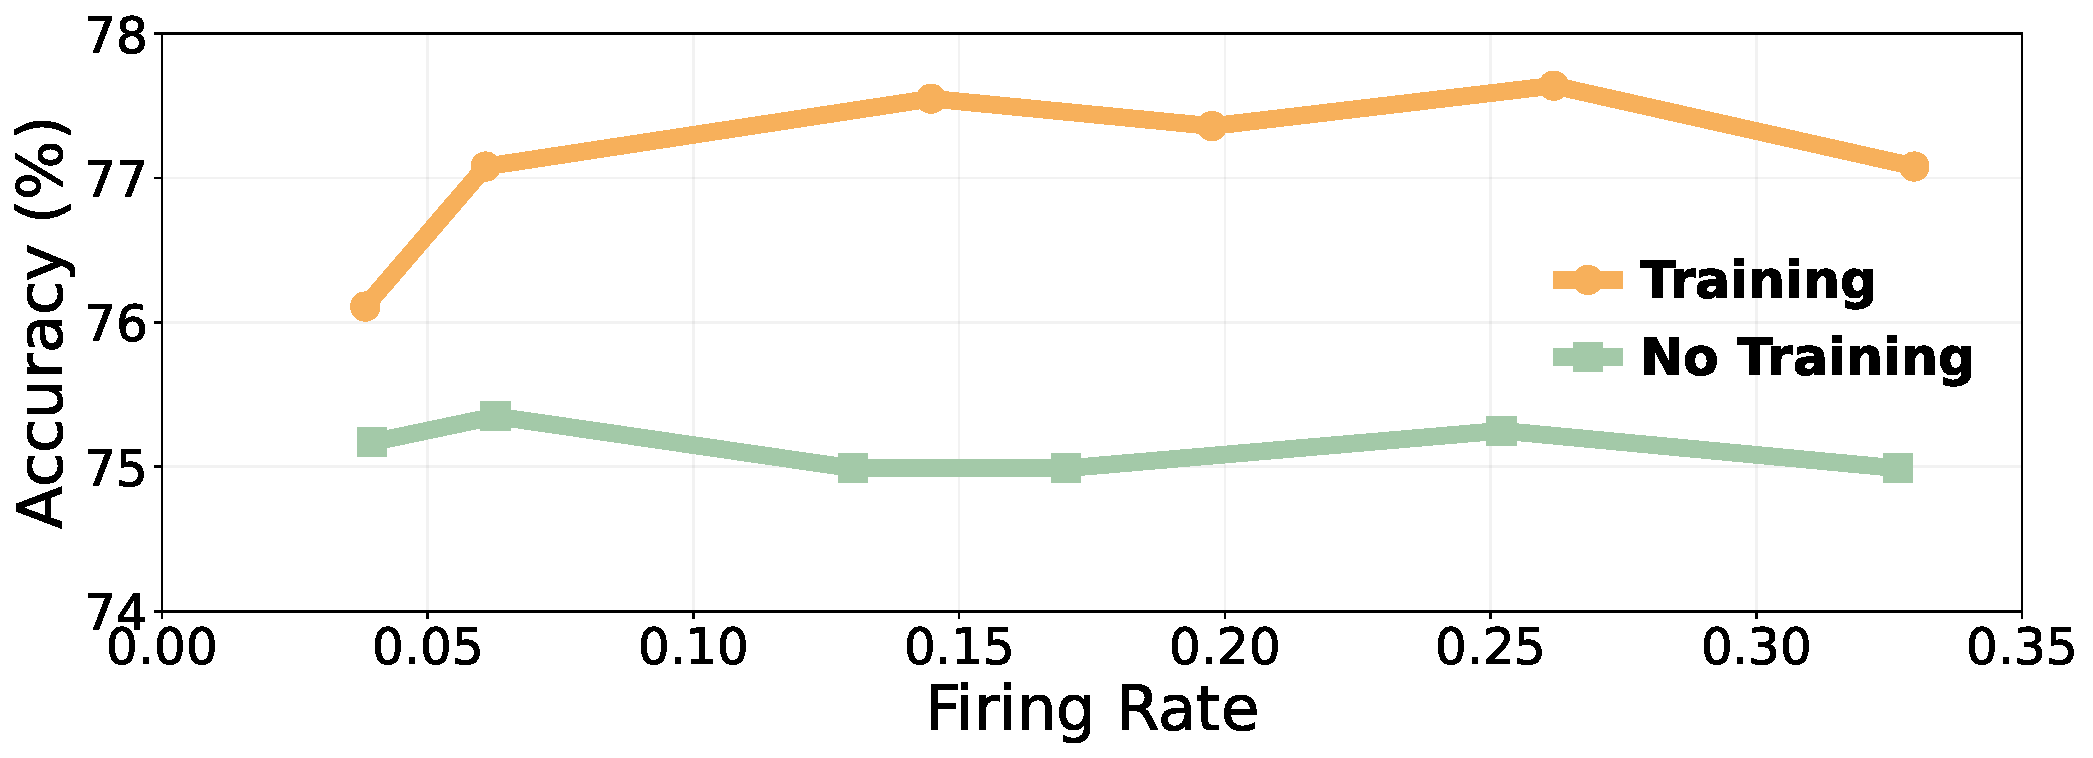
\includegraphics[width=0.99\linewidth]{fig/firing_rate_vs_accuracy_trsg.pdf}
  \caption{\textbf{Accuracy vs.\ firing rate under TrSG.}
  We sweep a sparsity loss~\cite{yan:2022} to match global firing rates and compare two settings:
  \emph{Training} (learn $V_{\text{thr}}$ and $\tau$ with TrSG) vs.\ \emph{No Training} (both frozen).}
  \label{fig:firing_rate_vs_accuracy_trsg}
\end{figure}

\subsection{Accuracy vs.\ Firing Rate}
\label{sec:acc_vs_firing_rate_trsg}

As shown in \cref{subsec:analysis_of_mpinit}, MP‑Init forms a Pareto front over firing rate.
A natural question is whether training internal parameters ($V_{\text{thr}}$, $\tau$) with TrSG merely increases spikes to boost accuracy.
To decouple these effects, we vary a sparsity regularization loss~\cite{yan:2022} that directly controls spike counts and evaluate accuracy across matched firing rates, comparing \emph{Training} (TrSG updates $V_{\text{thr}}$, $\tau$) to \emph{No Training} (both frozen).
As seen in \cref{fig:firing_rate_vs_accuracy_trsg}, the \textbf{Training} curve strictly dominates the \textbf{No Training} curve at all firing rates, indicating that the improvement stems from well‑adapted neuron dynamics rather than excessive spikes.
This is consistent with the threshold trajectories in \cref{fig:vthr_dynamics}, where layers evolve toward operating points that favor stable, informative spikes. 

\begin{table}[h]
\centering
\footnotesize
\begin{tabular}{ccccc}
\toprule
\textbf{MP-Init} & \textbf{TrSG} & \textbf{ACs / MACs(G)} & \textbf{Energy (mJ)} & \textbf{Acc (\%)} \\
\midrule
\ding{55} & \ding{55} & 1.03 / 0.14 & 1.57 & 75.58 \\
\ding{51} & \ding{55} & 1.01 / 0.14 & 1.57 & 76.20 \\
\ding{55} & \ding{51} & 1.13 / 0.14 & 1.68 & 77.13 \\
\ding{51} & \ding{51} & 1.12 / 0.14 & 1.67 & 77.68 \\
\bottomrule
\end{tabular}
\caption{\textbf{Energy at comparable firing rates.}
We report accumulate operations (ACs), multiply–accumulate operations (MACs), and the calculated energy costs.}
\label{tab:energy_calculation}
\end{table}

\subsection{Energy Cost}
Since firing rate tightly correlates with ACs (and thus energy), the analysis in \cref{subsec:analysis_of_mpinit,sec:acc_vs_firing_rate_trsg} can be viewed as an energy–accuracy trade‑off as well.
To quantify this, we measure ACs and MACs and compute energy following \cite{energy}; the results in \cref{tab:energy_calculation} show that, at similar firing rates (hence similar energy), training internal neuron parameters with TrSG yields consistently higher accuracy.
In short, TrSG improves accuracy at nearly the same energy cost, reinforcing that the gains come from better adaptation of $V_{\text{thr}}$ and $\tau$, not from increasing spike counts.


\begin{figure*}[ht]
  \centering
  \begin{subfigure}{0.995\linewidth}
      \begin{subfigure}{0.49\linewidth}
        \centering
        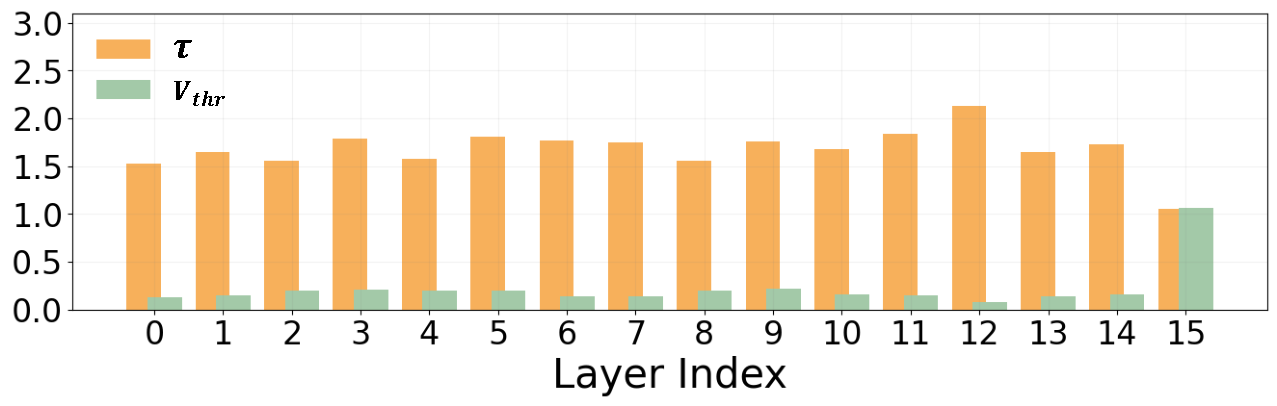
\includegraphics[width=0.99\linewidth]{fig/final_value_tau_thr_cifar100_resnet19_soft_reset_with_legend.pdf}
      \end{subfigure}
      \begin{subfigure}{0.49\linewidth}
        \centering
        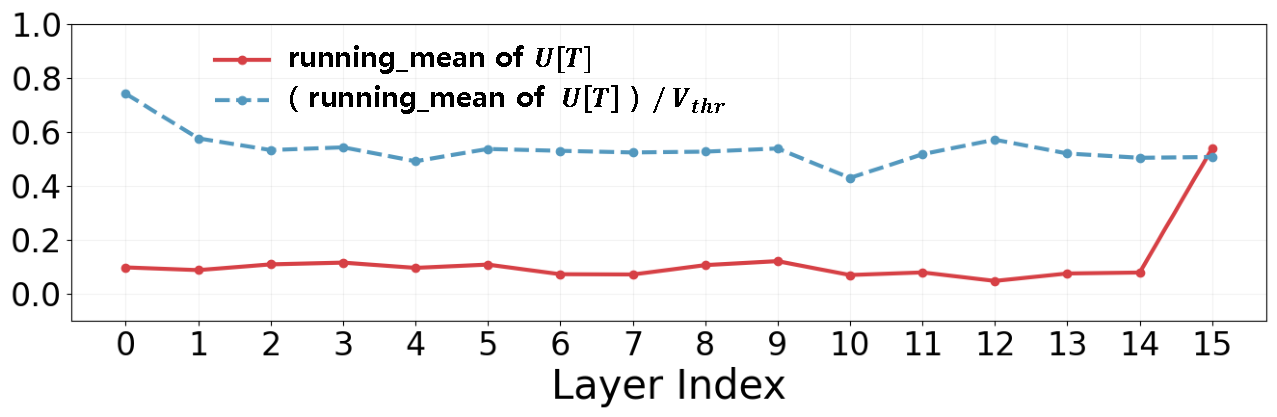
\includegraphics[width=0.99\linewidth]{fig/final_value_running_mean_cifar100_resnet19_soft_reset_with_legend.pdf}
      \end{subfigure}
      \caption{CIFAR100 (soft reset)}
      \label{fig:final_values_cifar100_softreset}
  \end{subfigure}
  \begin{subfigure}{0.995\linewidth}
      \begin{subfigure}{0.49\linewidth}
        \centering
        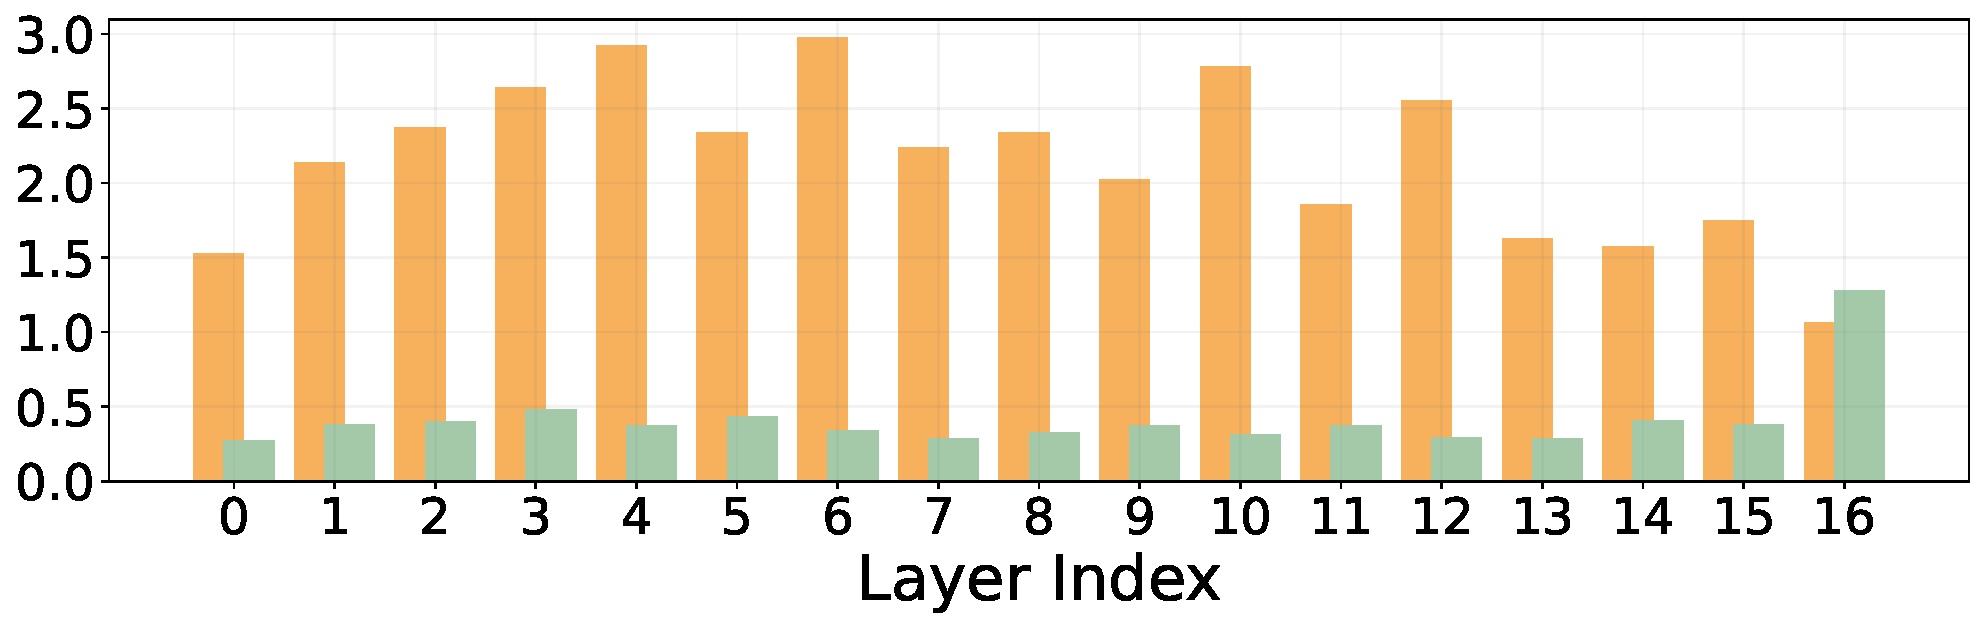
\includegraphics[width=0.99\linewidth]{fig/final_value_tau_thr_dvscifar10_resnet19_soft_reset.pdf}
      \end{subfigure}
      \begin{subfigure}{0.49\linewidth}
        \centering
        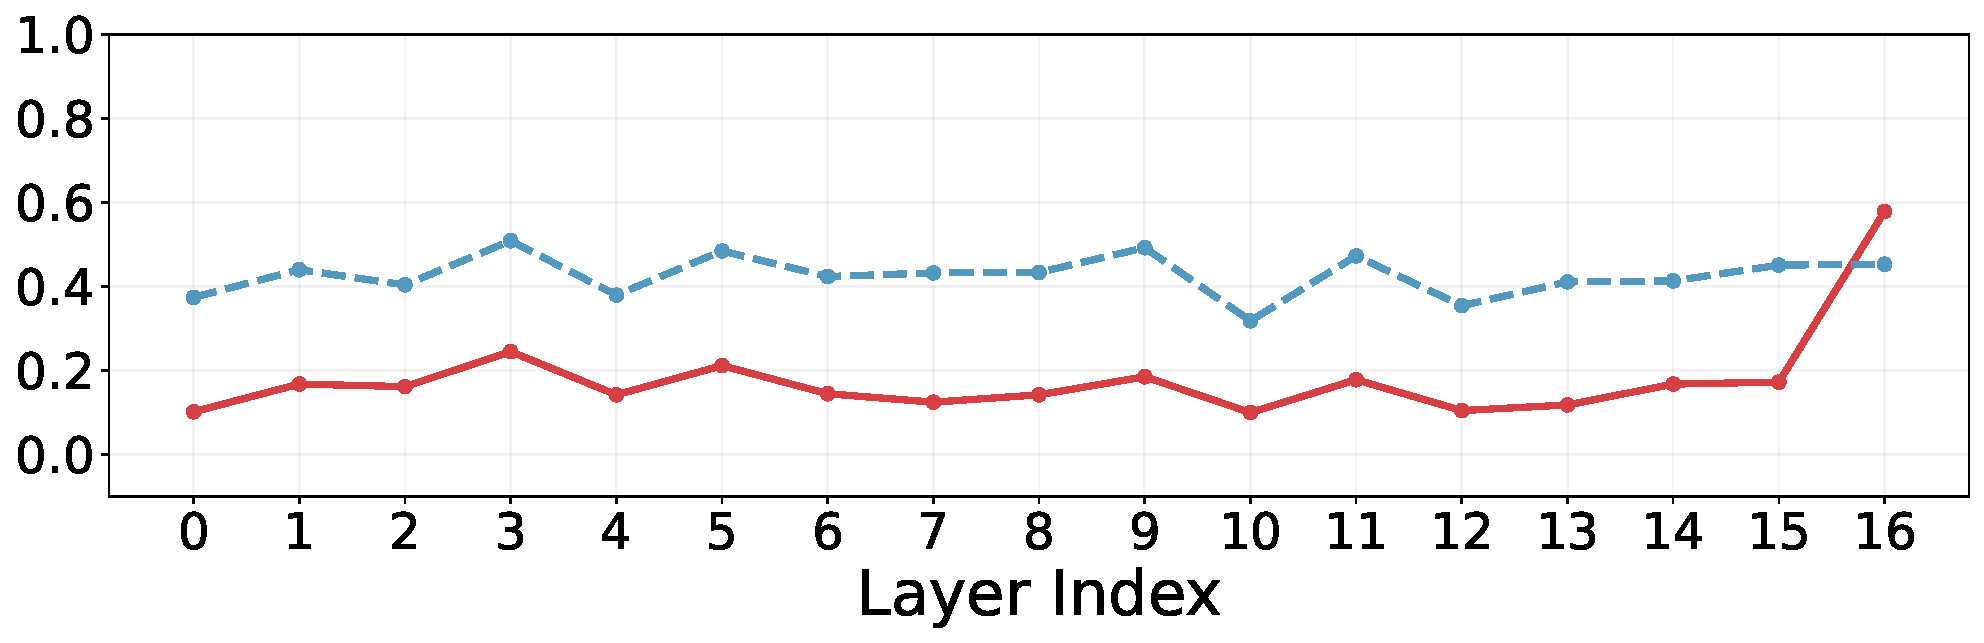
\includegraphics[width=0.99\linewidth]{fig/final_value_running_mean_dvscifar10_resnet19_soft_reset.pdf}
      \end{subfigure}
      \caption{DVS-CIFAR10 (soft reset)}
      \label{fig:final_values_dvscifar10_softreset}
  \end{subfigure}
  \begin{subfigure}{0.995\linewidth}
      \begin{subfigure}{0.49\linewidth}
        \centering
        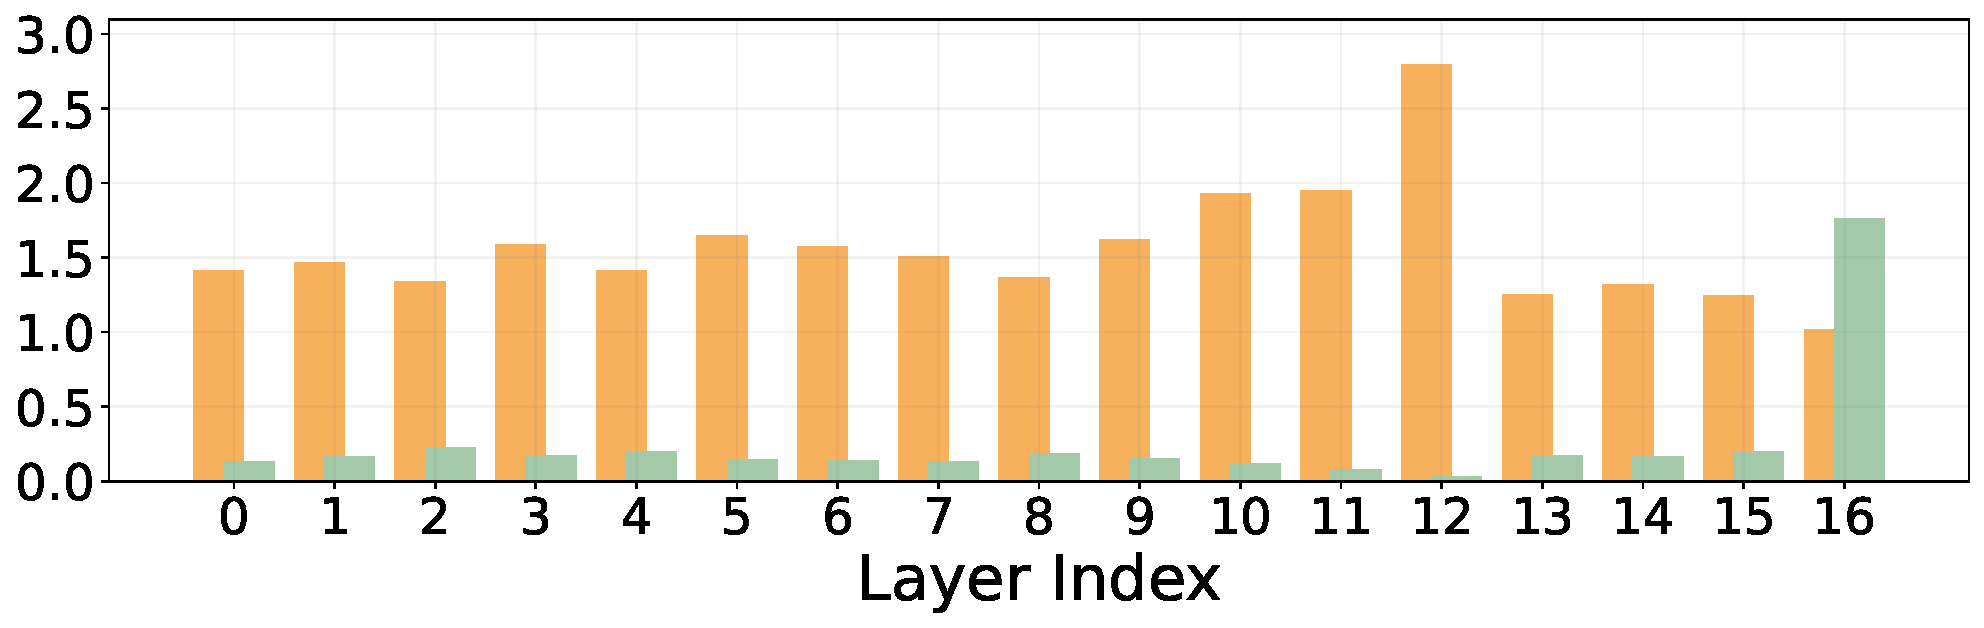
\includegraphics[width=0.99\linewidth]{fig/final_value_tau_thr_cifar100_resnet19_hard_reset.pdf}
      \end{subfigure}
      \begin{subfigure}{0.49\linewidth}
        \centering
        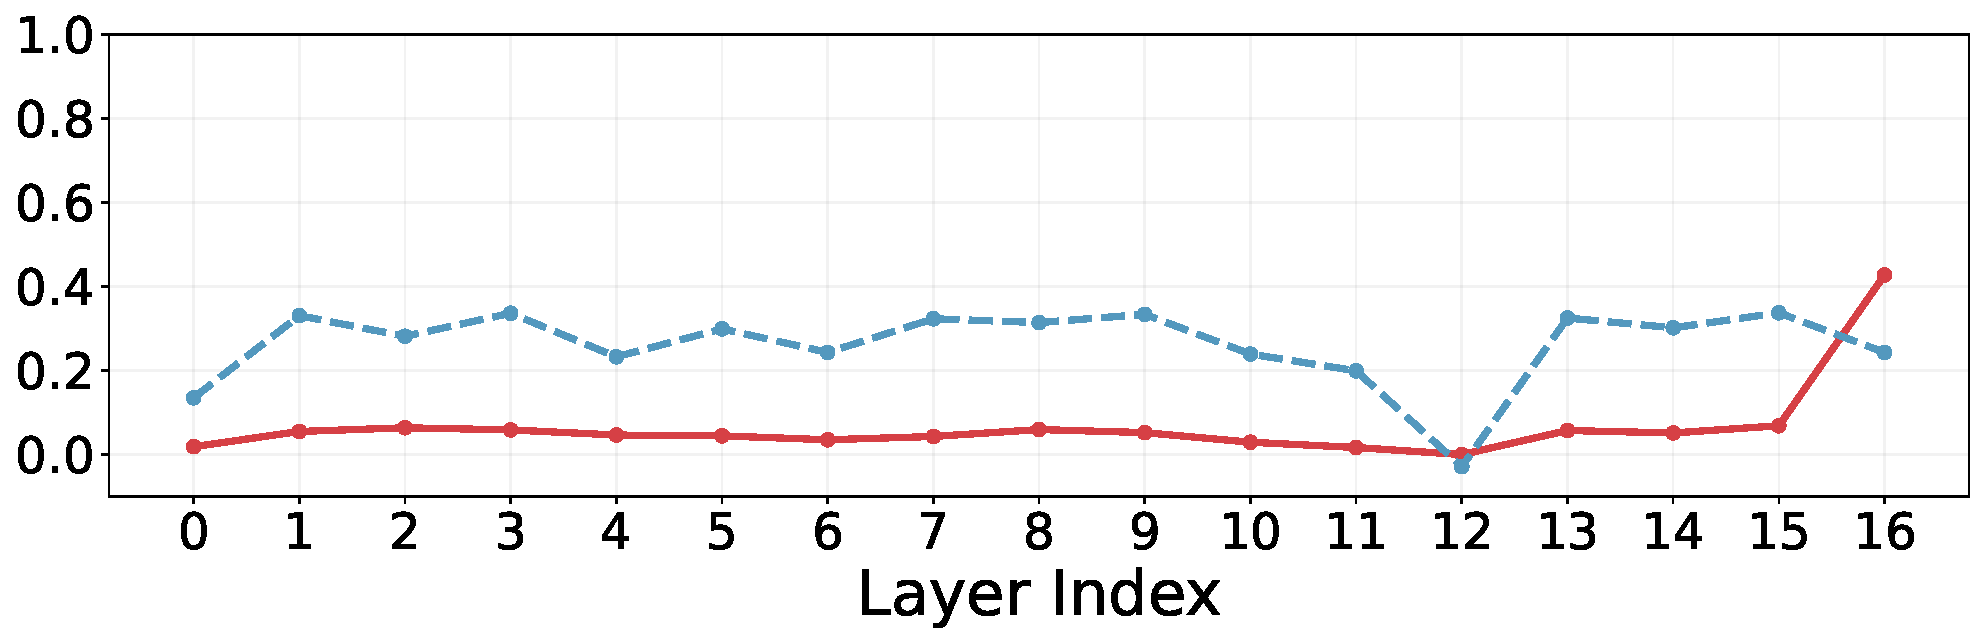
\includegraphics[width=0.99\linewidth]{fig/final_value_running_mean_cifar100_resnet19_hard_reset.pdf}
      \end{subfigure}
      \caption{CIFAR100 (hard reset)}
      \label{fig:final_values_cifar100_hardreset}
  \end{subfigure}
  \begin{subfigure}{0.995\linewidth}
      \begin{subfigure}{0.49\linewidth}
        \centering
        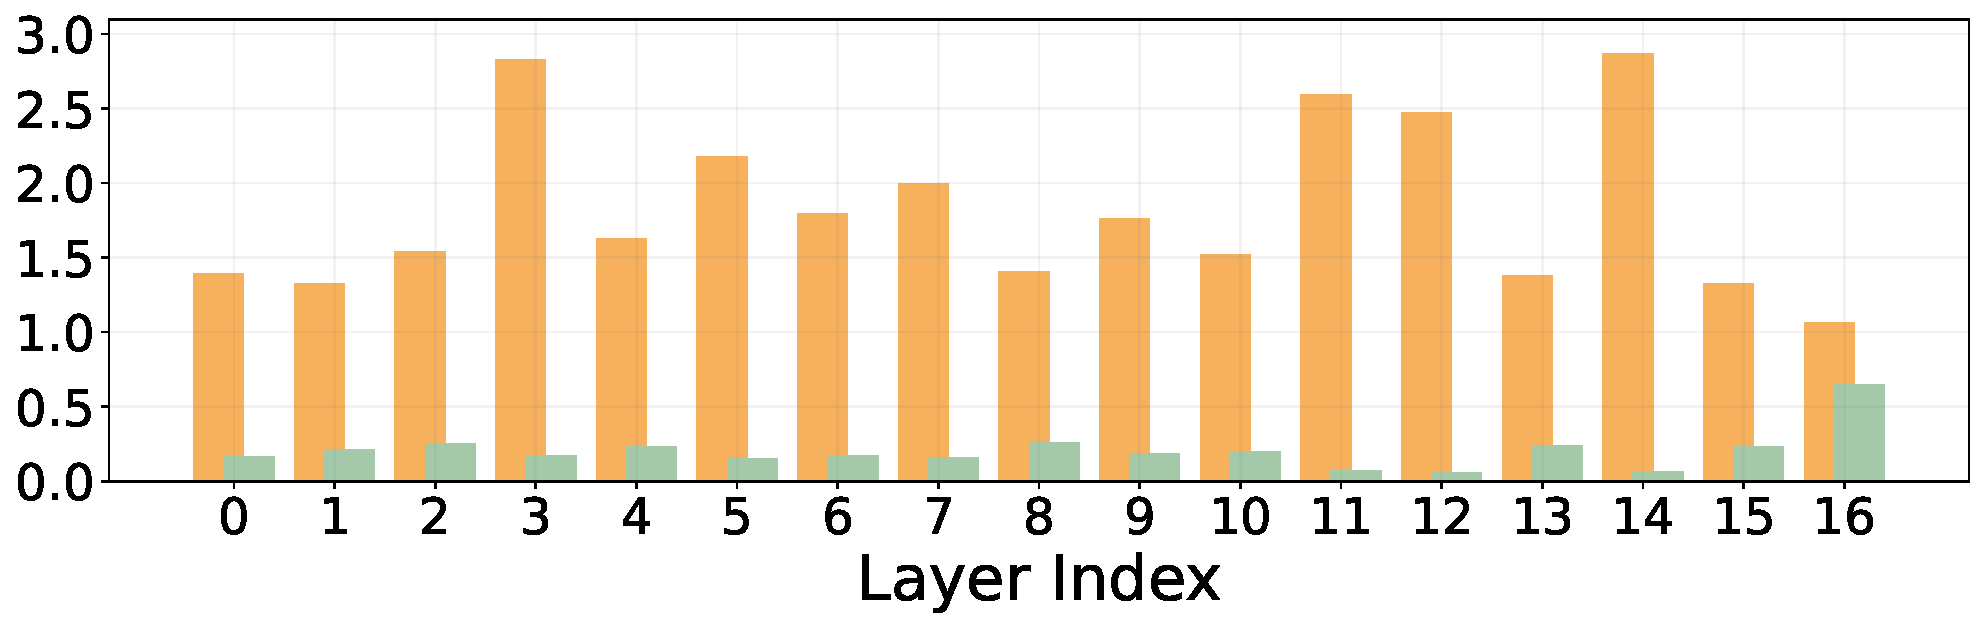
\includegraphics[width=0.99\linewidth]{fig/final_value_tau_thr_dvscifar10_resnet19_hard_reset.pdf}
      \end{subfigure}
      \begin{subfigure}{0.49\linewidth}
        \centering
        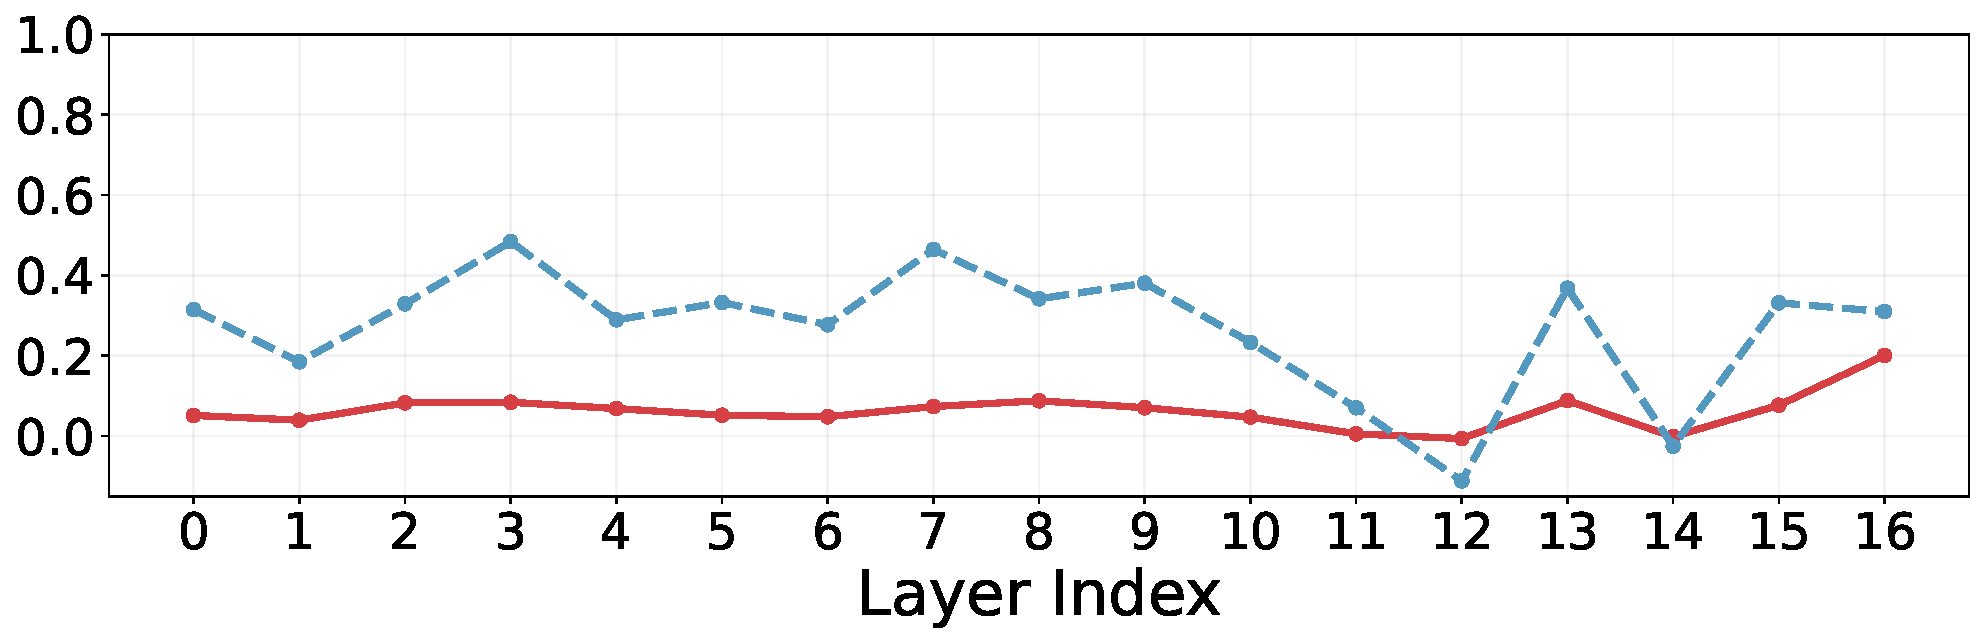
\includegraphics[width=0.99\linewidth]{fig/final_value_running_mean_dvscifar10_resnet19_hard_reset.pdf}
      \end{subfigure}
      \caption{DVS-CIFAR10 (hard reset)}
      \label{fig:final_values_dvscifar10_hardreset}
  \end{subfigure}
  \caption{The final values of \(V_{\text{thr}}\), \(\tau\), and the running mean of the membrane potential at the last timestep (\(U[T]\)) after training. ResNet-19 is trained on CIFAR100 (timestep = 4) and DVS-CIFAR10 (timestep = 10).}
  \label{fig:final_values}
\end{figure*}

\subsection{Final Values of Neuron Parameters}
\label{subsec:final_values_of_parameters}

In addition to learning the network weights, our approach also optimizes the neuron parameters \(\tau\) and \(V_{\text{thr}}\), while MP-Init tracks an internal running mean of the membrane potential at the last timestep, \(U[T]\). To investigate how these three quantities evolve through training, we visualize their final layer-wise values for both CIFAR100 and DVS-CIFAR10 in \cref{fig:final_values}, considering soft vs.\ hard resets.

\paragraph{Running Mean of \(U[T]\).}
The running mean of \(U[T]\) typically settles at about half of \(V_{\text{thr}}\) in the soft-reset case (\cref{fig:final_values_cifar100_softreset,fig:final_values_dvscifar10_softreset}) and roughly a quarter of \(V_{\text{thr}}\) for hard-reset neurons (\cref{fig:final_values_cifar100_hardreset,fig:final_values_dvscifar10_hardreset}). 
This pattern indicates that the average post-synaptic potential remains below the learned threshold in most layers yet remains sufficiently high to generate spikes as needed.

\paragraph{Threshold \(\boldsymbol{V_{\text{thr}}}\).}
Across both datasets and reset types, the learned \(V_{\text{thr}}\) commonly falls below 0.5 in earlier and intermediate layers, suggesting that moderate thresholds facilitate stable spiking activity.

\paragraph{Decay Constant \(\boldsymbol{\tau}\).}
We observe a consistent trend of \(\tau\) converging around 1.5--2.0 in most layers for CIFAR100, while on DVS-CIFAR10, \(\tau\) tends to reach even larger values (e.g., near 2.5--3.0). 
This discrepancy implies that dynamic event-driven data may benefit from neurons accumulating input more slowly, whereas CIFAR100’s static images require a shorter effective integration time.

\paragraph{Last-Layer Behavior.}
Interestingly, in the final layer on both datasets, \(\tau\) commonly drops close to 1, which makes it become a binary layer. The layer may act as a gating mechanism, helping the model to classify features decisively without excessive temporal integration.

\begin{figure}[h]
  \centering
  \begin{subfigure}{0.99\linewidth}
    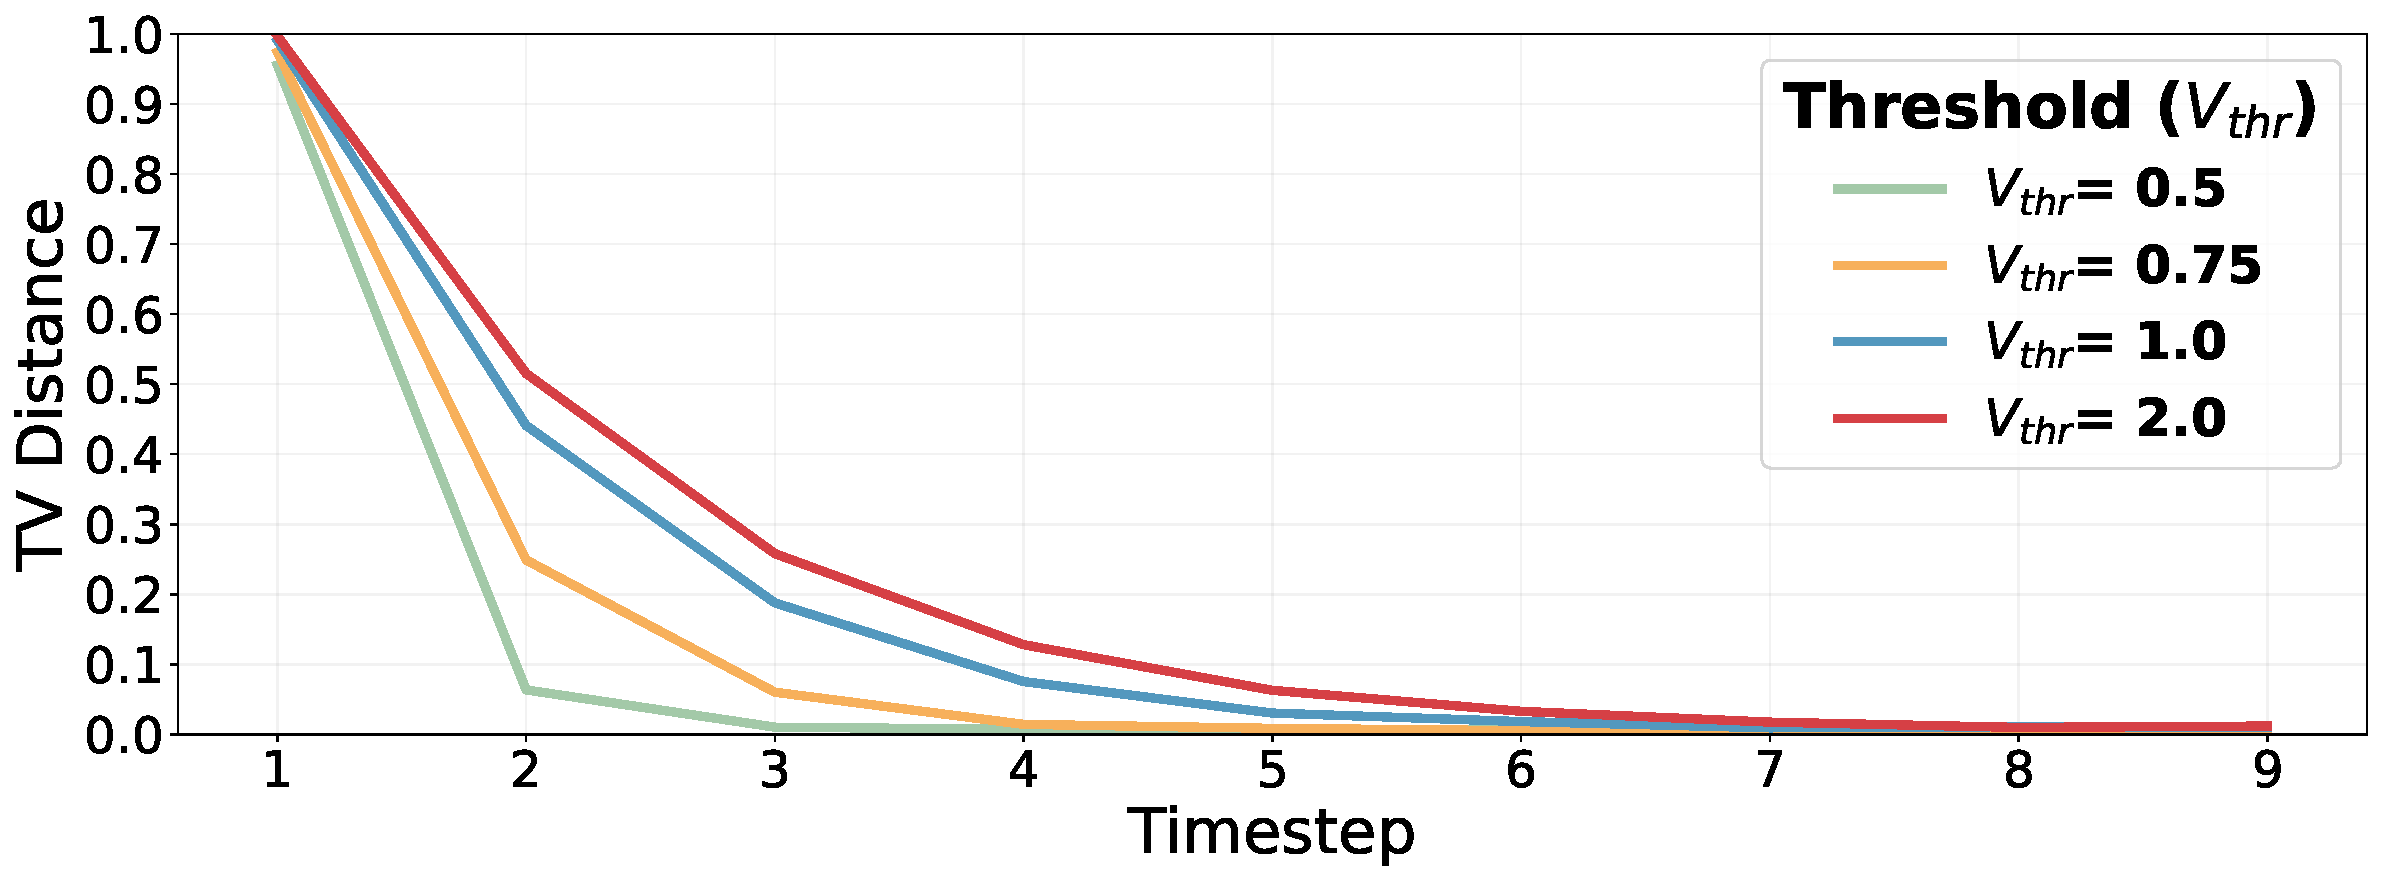
\includegraphics[width=0.99\linewidth]{fig/tv_distance_thr_plot.pdf}
    \caption{Impact of varying \(V_{\text{thr}}\) on convergence speed.}
  \end{subfigure}
  \hfill
  \begin{subfigure}{0.99\linewidth}
    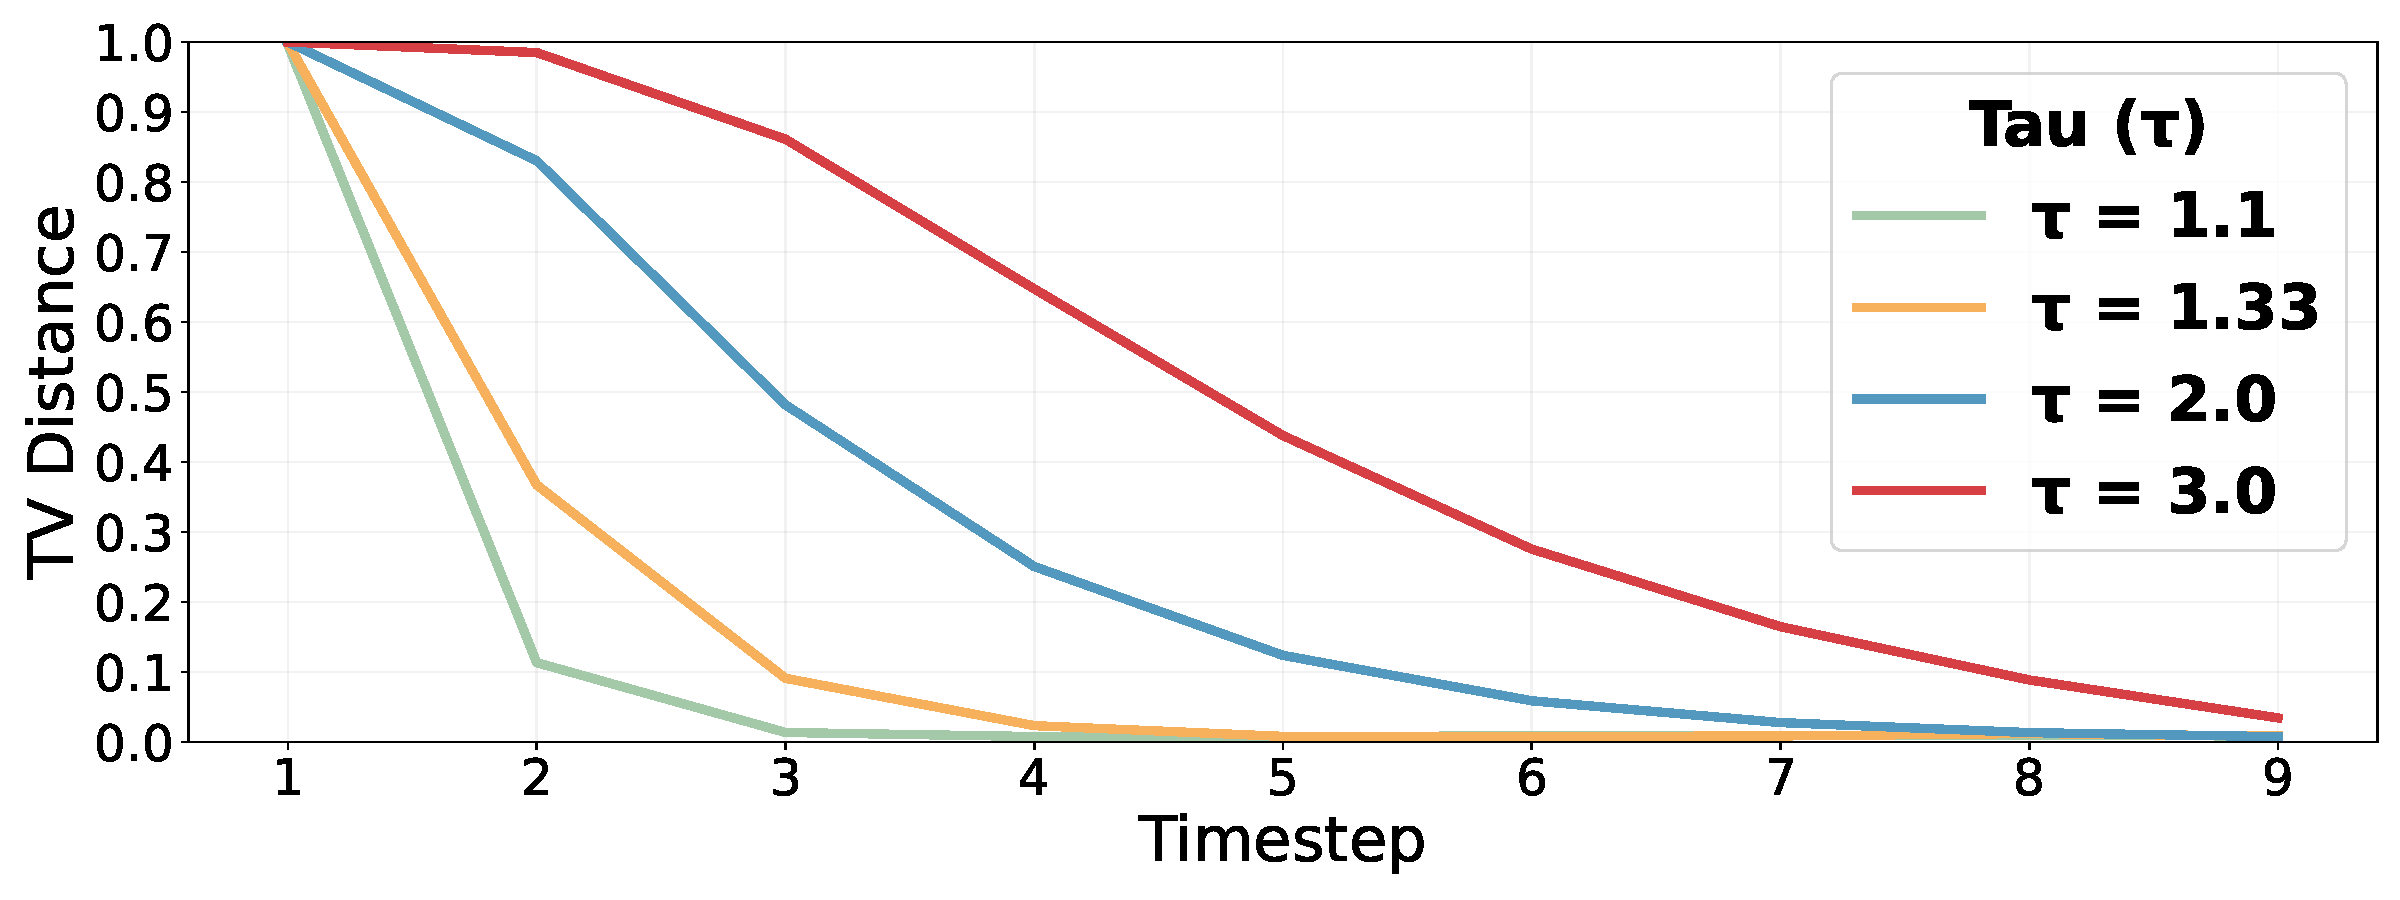
\includegraphics[width=0.99\linewidth]{fig/tv_distance_tau_plot.pdf}
    \caption{Impact of varying \(\tau\) on convergence speed.}
  \end{subfigure}
  \caption{TV distance of membrane potential distribution between timestep 10 and previous timesteps, illustrating the effects of altering the threshold \(V_{\text{thr}}\) (Left) or the time decay constant \(\tau\) of the LIF neuron (Right). The input is randomly generated from a Gaussian distribution.}
  \label{fig:tv_norm}
\end{figure}

\subsection{Convergence Rate of Membrane Potential}

To analyze the factors influencing the convergence rate described in Theorem 1, we conduct a mathematical analysis complemented by simple experiments, revealing that the time decay constant \(\tau\) and the threshold voltage \(V_{\text{thr}}\) play pivotal roles in determining the convergence speed, thereby influencing the TCS problem.

As outlined in \cref{eq:minimorization_condition} and \cref{eq:convergence_speed}, Doeblin’s Minorization Condition ensures not only the convergence of distributions but also provides insights into the convergence speed. Consider the uniform measure \(\mu\), which represents a uniform distribution over the interval \([u^{-}, u^{+}]\). For simplicity, let \(U[t-1] = 0\), such that \(U[t] = \frac{1}{\tau} I_{\text{in}}[t]\). Under these assumptions, \cref{eq:minimorization_condition} can be expressed as:

\begin{equation}
    P\left(U[t] = \frac{1}{\tau} I_{\text{in}}[t] \in A\right) \geq \epsilon \mu(A),
\end{equation}

From this expression with the Assumption. 1, it becomes evident that decreasing \(\tau\) increases the maximum permissible value of \(\epsilon\), which, in turn, accelerates the convergence speed as per \cref{eq:convergence_speed}. Similarly, reducing the threshold \(V_{\text{thr}}\) results in the membrane potential reaching the threshold more frequently, triggering resets. This frequent resetting narrows the range \([u^{-}, u^{+}]\) of the membrane potential, thereby increasing \(\epsilon\) and further accelerating convergence.

We conduct experiments utilizing soft reset LIF neurons with Gaussian input to validate the theoretical findings. The parameters \(V_{\text{thr}}\) and \(\tau\) are varied, and the TV distance~\cite{rosenthal:1995} is computed between the distribution at each timestep and the final distribution, as illustrated in \cref{fig:tv_norm}. The results confirm that smaller values of \(V_{\text{thr}}\) and \(\tau\) can alleviate the TCS problem. However, it is crucial to note that setting these parameters to excessively low values is not universally advantageous.

For instance, a threshold \(V_{\text{thr}}\) that is too low can result in excessive firing rates, leading to unstable network dynamics. Similarly, an overly small \(\tau\) degrades the neuron’s ability to accumulate membrane potential over time, effectively reducing its behavior to binary quantization. Therefore, the selection of \(V_{\text{thr}}\) and \(\tau\) requires a careful balance to achieve both rapid convergence and stable network dynamics.

This analysis might establish a connection between MP-Init and TrSG. Rather than relying on manual tuning, training \(V_{\text{thr}}\) and \(\tau\) as learnable parameters within the network can be more effective. As shown in \cref{subsec:final_values_of_parameters}, TrSG successfully optimizes \(V_{\text{thr}}\) and \(\tau\), leading them to moderately low values and achieving superior accuracy.